\documentclass{article}
\usepackage[utf8]{inputenc}
\usepackage[margin=1in]{geometry}
\usepackage{notes}
\usepackage{tikz-cd}

\setcounter{section}{-1}

\title{Math 101 Notes}
\author{Henry Cerbone, Max Guo, Sarah Chin}
\date{Spring 2021}

\begin{document}

\maketitle

\tableofcontents

\section{Introduction}

These notes are taken by the CA's, and they may have significant overlap with the notes posted on various locations on Canvas. Feel free to use these notes for supplementing your learning!

\section{Lecture 1: 01/25/2021}

\subsection{The Raisin Game}

You and your friend start with $n$ raisins, where $n$ is a positive integer (e.g. $1, 2, \dots$). You decide to play a game with your friend where you each take $1, 2, 3,$ or $4$ raisins when it is your turn. The person who takes the last raisin wins. \\

How do we come up with a strategy for this game? After playing a few games, you might realize that the number $5$ is quite special. If your friend reaches the number $5$ (and then it's your turn), then unfortunately, no matter how many raisins you take, your friend can take the last raisin by taking the remaining raisins.\\

After playing some more, we realize that for the numbers $6, 7, 8,$ and $9$, whoever goes first wins! The first player can force the next player to start with $5$ raisins, which results in a win for the first player.\\

At this point, we might form the following conjecture:

\begin{conjecture}
The second player has a winning strategy iff (if and only if, or ``exactly when") at the start the number of raisins is a multiple of $5$.
\end{conjecture}

\begin{proof}
First we do the ``if" direction. Suppose the number of raisins is a multiple of $5$. Then the first player takes some number of raisins $x$, where $x$ is $1, 2, 3,$ or $4$. Then the second player can take $5-x$ raisins, and the remaining number of raisins is another multiple of $5$. Thus, the second player can continue to force the first player to start at smaller and smaller multiples of $5$ until they reach the number $5$. The first player then takes some number of raisins, and as discussed above the second player wins no matter how many the first player takes.\\

Next we do the ``only if" direction. Suppose the number of raisins is not a multiple of $5$. Then the first player can win by taking a number of raisins that leaves a multiple of $5$, so the argument above shows you have a winning strategy.
\end{proof}

Here is an example of some conjectures that are not always true. The mathematician Leonhard Euler stated that:
\begin{conjecture}
$n^2 + n + 41$ is prime for $n = 0, \dots, 39$.
\end{conjecture}
This might lead one to think that the above is true for all $n\geq0$, but we can provide a counterexamples for things outside this range such as $40^2 + 40 + 41$. (You will learn about techniques to prove that for $n>39$ Euler's polynomial is not prime later in the course).
Here is another from Fermat
\begin{conjecture}
$2^{2^n} + 1$ is prime for $n = 0, 1, 2,3,4$ and composite for $n=5$.
\end{conjecture}


\subsection{Fundamentals}

Some important definitions!

\begin{definition}[Evenness]
An integer $n$ is \textit{even} if $n = 2k$ for some integer $k$.
\end{definition}

These ``if"'s should actually be ``iff"'s (if and only if). However, in definitions, we usually assume that if means iff.

\begin{definition}[Oddness]
Correspondingly, an integer $n$ is \textit{odd} if $n = 2k+1$ for some integer $k$. 
\end{definition}

\begin{definition}[Divisibility]
An integer $m$ \textit{divides} an integer $n$, written $m|n$, if $n = mk$ for some integer $k$.
\end{definition}

\begin{definition}[Casework]
Sometimes when we write a proof, we want to split up the possibilities to prove it in ``cases".
\end{definition}

\begin{example}
Prove that $n(3n + 1)$ is always even. 
\end{example}

\begin{proof}
We begin with a generality statement. This means we pick an arbitrary integer $n$ and then proceed with our proof. Because we just picked an arbitrary number, our proof will still hold. We can split this into two cases: when $n$ is even, when $n$ is odd.\\

\textbf{Case 1}: $n$ is even.\\

If $n$ is even we have that $n = 2k$ for some integer k, so 
\[
n(3n +1) = 2k(3n + 1),
\]
which is even.\\

\textbf{Case 2}: $n$ is odd.\\

If $n$ is odd, we can write that $n = 2k+1$ for some integer $k$, so 
\[
n(3n+1) = n(6k+4) = 2(n(3k+2)),
\]
which is even.
\end{proof}


\section{Lecture 2: 01/27/2021}

\subsection{Mathematical Induction}

Today we'll introduce two types of induction: regular (``weak") induction and strong induction.

\begin{example}
What is $1 + 2 + \dots + n$?
\end{example}

We can think about representing this visually by using a triangle. This would look (sort of) like:
\begin{table}[h]
    \centering
    \begin{tabular}{c c c}
        $\bigcdot$ & & \\
        $\bigcdot$ & $\bigcdot$ & \\
        $\bigcdot$ & $\bigcdot$ & $\bigcdot$\\
    \end{tabular}
\end{table}

This should seem reminiscent of a right triangle! We know how to find the area of this (a visual proof is given in Figure \ref{fig:rect} below). In this proof, we think of our triangle as half a rectangle. We can use this same intuition to help us here. 

\begin{figure}[h]
    \centering
    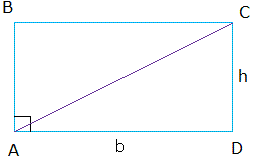
\includegraphics[scale=.5]{notes/images/rect.png}
    \caption{Rectangle}
    \label{fig:rect}
\end{figure}

We can now think of finding the area of the square which will have side length $n$ and $n+1$. We then see that we can express the summation of our sequence as 
\[
2(1 + 2 + \dots + n) = n(n+1)
\]
which can be simplified to give our desired result of 
$$
\frac{n(n+1)}{2}.
$$

We can give a second proof to this:
\begin{proof}
Let $n$ be a natural number (positive integer). Let 
\begin{align*}
  s_n &= 1+2+ \dots +(n-1)+n \\
  s_n &= n+ (n-1) +\dots + 2+1
\end{align*}
Adding the previous two lines gives
\[2s_n  = (n+1)+(n+1)+\dots (n+1)+(n+1)\]
So we have:
\begin{align*}
    2s_n &= n(n+1)\\
    \implies 2(1+2+\dots +(n-1)+n) &= n(n+1)
    \\
    \implies 1+2+\dots +(n-1)+n &= \frac{n(n+1)}{2}
\end{align*}

\end{proof}

Finally, we can do an inductive proof by induction on $n$ for all natural numbers $n$:
\begin{proof}
In induction, we always have two steps. First, the base case, which in this example is $n =1$:
\begin{enumerate}
    \item \textit{Base case}. When $n = 1$, $1 = \frac{1(2)}{2}$.
    \item \textit{Induction step}. Let's suppose that our formula works for some natural number $n$. Now we shall show that it will work for $n+1$ as well. We want to show that:
    \[
    1 + 2 + 3 + \dots + n + (n+1) = \frac{(n+1)(n+1+1)}{2}.
    \]
    
    Note that on the left, we have the expression $(1 + 2 + \dots + n) + n+1$, so we can apply the induction hypothesis:
    \begin{align*}
        \frac{n(n+1)}{2} + n+1 &= \frac{(n+1)(n+2)}{2},
    \end{align*}
    which is what we wanted to show.
\end{enumerate}
\end{proof}

Let's try another example.
\begin{example}
Prove that $8 | 3^{2m-1} + 5$ for all natural numbers $m$.
\end{example}
\begin{proof}
We prove the base case first. For $m = 1$, we have that $8 | 3 + 5 = 8$, which is true.\\

For the inductive step, we assume that $8 | 3^{2m-1} + 5$ is true. We wish to show that:
\[
8 | 3^{2(m+1) - 1} + 5.
\]
This can be shown by recognizing the following:
\begin{align*}
    3^{2(m+1) - 1} + 5 &= 3^{2m+1} + 5\\
    &= 9 \cdot 3^{2m-1} + 5\\
    &= (8+1)\cdot 3^{2m-1} + 5\\
    &= 8\cdot 3^{2m-1} + 3^{2m-1} + 5\\
    &= 8\cdot 3^{2m-1} + 8k\\
    \implies 8 &| 3^{2(m+1) - 1} + 5,
\end{align*}
where we know $3^{2m-1} + 5$ can be written as $8k$ due to the inductive hypothesis. Thus, the proof is complete.
\end{proof}

So far, we have been talking about regular induction. Now, let's take a look at strong induction. In regular induction, we have been showing that our inductive step is true for our base case plus one. In strong induction, we want to show that the statement is true for all numbers up to some $k$.

\smallbreak

Here is an example of strong induction.
\begin{theorem}
Every integer $n > 1$ has a prime factor.
\end{theorem}
We can consider doing this by using regular induction
\begin{example}
\begin{align*}
    49 &= 7 \cdot 7 \\
    50 &= 2 \cdot 25 = 2 \cdot 5 \cdot 5.
\end{align*}
From the above we see that if we go to the next number, our case suddenly looks different (there are three prime factors!). This is a hint that regular induction may not be a good choice here. 
\end{example}
We can prove it by strong induction instead:
\begin{proof}
Using strong induction (it's a courtesy to your reader to announce when you'll be using strong induction).
\begin{enumerate}
    \item \emph{Base Case : } $\alpha$ has the prime factor $\alpha$ (where $\alpha$ is prime). 
    \item \emph{Induction Step: } Suppose, for some $k>1$, that $2, \dots, k$ have a prime factor. We want to show that $k+1$ has a prime factor.
    \item \emph{Case 1 : } If $k+1$ is prime, then it has itself as a prime factor. 
    \item \emph{Case 2 : } Otherwise, it has some factor $d$ other than $1$ and $k+1$. By the induction hypothesis, since $1 < d < k+1$, $d$ has a prime factor $p$. So, $p$ is a prime factor of $k + 1$.
\end{enumerate}
\end{proof}

A final example of strong induction:
\begin{example}
A rectangular chocolate bar is made up of $N$ smaller $(1\times 1)$ squares of chocolate. You are going to break the chocolate bar into $1\times1$ squares by breaking along the straight grooves between the rows and columns of squares. Show by strong induction on $N$ that, no matter how you do the breaking, it will take you $N-1$    ``breaks". (Why is weak induction not enough?)
\end{example}

\begin{proof}
For the base case, we can simply take $N=1$, the $1\times1$ chocolate bar, and indeed it takes $1-1 = 0$ breaks to achieve the result. For the inductive step, we can assume that the statement is true for all chocolate bars up to size $N$. Now take a chocolate bar of size $N+1$. With some break, we will achieve two chocolate bars of size $a$ and $b$, where $a < N+1$, $b < N+1$, and $a+b = N+1$. By strong induction, it takes $a-1$ breaks for the first bar, $b-1$ breaks for the second bar, and thus a total of $a-1 + b-1 + 1$ (the last $+1$ is for the first break), which is $a+b-1 = N-1$ breaks total, which is what we wanted to prove.
\end{proof}
\section{Lecture 3: 02/01/2021}

\subsection{Types of Proof}
Today we will look at three ways to show an if-then statement : direct, contrapositive, and contradiction.
\smallbreak

From the Preparatory Problem Set:
\begin{itemize}
    \item Statement: If $ab > 0$, then $a > 0$ and $b > 0$. (\textbf{False})
    \item Converse: If $a > 0$ and $b > 0$, then $ab > 0$. (\textbf{True})
    \item Contrapositve: If it's not true that $a > 0$ and $b > 0$, then it's not true that $ab > 0$. (\textbf{False})
\end{itemize}

Recall that ``$P$ iff $Q$" means that ``If $P$, then $Q$" and "If $Q$, then $P$". In other words,
\[
P \implies Q \; \; AND \; \; Q \implies P.
\]

Note: \textit{a statement is equivalent to its contrapositive}!

\begin{example}
Negate the following statements:
\begin{enumerate}
    \item $x > 0$ or $x$ is rational.
    \item Every country in the U.S. as at least $5$ farms.
\end{enumerate}
\end{example}

\begin{proof}\quad
\begin{enumerate}
    \item $x \le 0$ AND $x$ is irrational.
    \item There exists (we use the symbol $\exists$ often) a country in the U.S. with $< 5$ farms.
\end{enumerate}
\end{proof}

There is also a shorthand symbol for ``for all", denoted by $\forall$.

We given an example of a direct proof. 
\begin{example}
Prove that, if $a$ and $b$ are integers and $a | b$, then $a | b^2$.
\end{example}

\begin{proof}
Suppose $a$ and $b$ are integers and $a | b$. Then $b = ak$ for some integer $k$. To prove that $a | b^2$, we want to show that $b^2 = ak'$ for some $k'$. We can take $k' = ak\cdot b$, which proves the statement.
\end{proof}

Now we'll give an example of a contrapositive proof (proving the contrapositive!)

\begin{example}
Any integer whose square is even must be even. (In other words, if $n$ is an integer such that $n^2$ is even, then $n$ is even). Give a contrapositive proof of the claim.
\end{example}

\begin{proof}
Let $n$ be an integer. Suppose $n$ is odd. Then, $n = 2k+1$ for some integer $k$. So $n^2 = 4k^2 + 4k + 1 = 2(2k^2 + 2k) + 1$ is odd. This proves the contrapositive.
\end{proof}

Tangential note: before we had assumed that every integer was either even or odd. However, now we know how to prove it! We can use the division algorithm (theorem) that states:

\begin{theorem}
For any integer $a$ and positive integer $b$, there exist integers $q$ and $r$ such that $a = bq + r$ and $0 \le r < b$.
\end{theorem}

Since this is true for all $a$ and $b$, we can take $b = 2$, which shows that $r = 0$ or $1$ for all integers (which implies that every integer is either even or odd - convince yourself!).

\begin{example}
Let $m$ and $n$ be integers. If $m$ and $n$ have different parity, then their sum is odd.
\end{example}

\begin{proof}
Let $m, n$ be integers with different parity. We use the term "without loss of generality" (WLOG) to cover identical cases. In this case, because $m+n$ is the same as $n+m$, we can say: WLOG let $m$ be even and $n$ be odd.
\end{proof}

Finally, we do a proof of contradiction. In a contradiction proof of ``If $P$, then $Q$", we suppose that $P$ is true and $Q$ is false. We then try to work towards some contradiction. The advantages of this method is that you start off with more information, but the disadvantage is that you don't know where you are going - you just want to find some sort of contradiction.

\begin{example}
Prove that $\sqrt{2}$ is irrational.
\end{example}

\begin{proof}
Suppose for the sake of contradiction that $\sqrt 2$ is rational. Then $\sqrt 2 = \frac a b$ where $a, b$ are integers that share no common divisors $ > 1$. Therefore $a = b\sqrt 2$, and $a^2 = 2b^2$. Then $a^2$ is even, which means that $a$ is even. Then $a = 2k$ for some integer $k$. Plugging this in, we have $4k^2 = 2b^2$, so $b^2 = 2k^2$. Then $b^2$ is even, so $b$ is even. This is a contradiction, since $a$ and $b$ share the common divisor $2$ although we had assumed they shared no common divisors.
\end{proof}
\section{Lecture 4: 02/03/2021}
Today we will be talking about sets! As you go forward in math, you will repeatedly see the fundamentalness of sets. Here are some sets you may be familiar with:
\begin{itemize}
    \item $\N$ which is the set of natural numers (positive integers)
    \item $\Z$ which is the set of integers
    \item $\Q$ which is the set of rational numbers
    \item $\R$ which is the set of real numbers
    \item $\C$ which is the set of complex numbers
\end{itemize}
\subsection{Some Notation}
There are two ``flavors" of notation for specifying a set.
\begin{enumerate}
    \item The first is when we want to apply a condition. This takes the form of 
    $$
    \{w \in \Z \mid 3 \le w < 6 \} = \{3, 4, 5\}
    $$
    where $\mid$ means ``such that".
    \item Another form of notation looks like
    $$
    \left\{\frac{1}{k} \mid k \in \Z\right\}
    $$
\end{enumerate}
The difference between these two is the order of the variable. In the first we have $\{\text{variable} \; \mid \text{condition}$ and in the second we have a the variable and then the relation. 
\begin{example}
True or false. 
\begin{enumerate}
    \item $\{n \in \Z : 2 \mid n \} = \{2k : k \in \Z \}$ We see that this is true as both sides are the even integers.
    \item $\{2n \mid n \in \Z\} = \{-2n \mid n \in \Z\}$ These are again both describing even integers so the equality holds.
\end{enumerate}
\end{example}
\subsection{Set Operations}
Before talking about set operations, it is important to go over a particular set relation. We can draw the intuition for this from our knowledge of Venn diagrams. This is made more clear in the figure \ref{fig:sets}.
\begin{figure}[h]
    \centering
    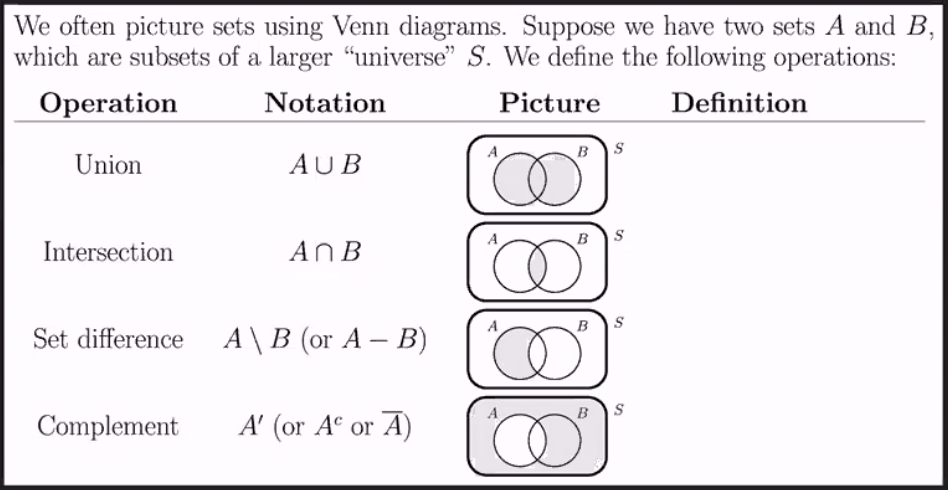
\includegraphics[scale=.4]{notes/images/set-relations.PNG}
    \caption{Set Relations as Venn Diagrams}
    \label{fig:sets}
\end{figure}
Filling in the definitions for Figure \ref{fig:sets} we have:
\begin{enumerate}
    \item $\{x \mid x \in A \; \text{or} \; x \in B\}$
    \item $\{x \mid x \in A \; \text{and} \; x \in B\}$
    \item $\{x \in A \mid x \not\in B\}$
    \item $\{S\setminus A\} = \{x \in S \mid x \not\in A\}$
\end{enumerate}
If we want to prove $x \in A \cap B$, show $x \in A$ and $x \in B$.
\begin{definition}
Let $S, T$ be sets. We say $S$ is a \textit{subset} of $T$, written $S \subseteq T$, if every element of $S$ is also an element of $T$. We say $S$ is a proper subset of $T$, $S \subsetneq T$, if $S \subseteq T$ and $S \neq T$. 
\end{definition}
\subsubsection{Interesting Question!}
Is the empty set an element of every set? We can parse this question as : If $x \in \phi$, is $x \in S$. We can think of a similar (perhaps not obviously related) question. If a person is drinking alcohol, they must be $\geq 21$. This statement has a counterexample as we can find a counterexample (a 19 year old drinking alcohol). Turning back to our original question, we see that $x \in \phi$ is always false. Therefore, we have that the statement itself holds. When things are true for this reason, we say that things are \textit{vacuously} true. This means that the antecedent (in this case $x \in \phi$ can never be satisfied. 
\subsection{Set Inclusion}
Consider the following example,
\begin{example}
Let $A = \{12n \mid n \in \Z\}, B = \{k \in \Z \mid k \; \text{is even}\}\text{, and } C = \{3j \mid j \in \Z\}$. Prove using the definitions of subset and intersection that $A \subseteq B \cap C$. 
\begin{proof}
Let $x \in A$. Then, $x = 12n$ for some $n\in \Z$. We can rewrite $x = 2(6n)$, so $x$ is even sine $6n \in \Z$ so $x\in B$. We can also rewrite $x = 3(4n)$, so x $\in C$. By definition of intersection, $x \in B \cap C$.
\end{proof}
\end{example}
\subsection{Set Equality}
In proving set equality, we rely on the fact that if the left is a subset of the right and vice versa, then our sets are equal. To further show this, we consider the following example.
\begin{example}
$(A \cap B) \cup (A \setminus B) = A$
\begin{proof}
Proving the first inclusion $(\subseteq)$, let $x \in (A \cap B) \cup (A \setminus B)$. By the definition of the union, we have that $x \in A \cap B$ or $x \in A \setminus B$. In either case, $x \in A$ relying on the definition of the the intersection and set difference. 
\smallbreak
Now we need to prove the other direction $\supseteq$. Let $x \in A$. Either $x \in B$ or $x \not \in B$.
\begin{itemize}
    \item If $x \in B$, then $x \in A \cap B$. 
    \item If $x \not\in B$, then $x \in A \setminus B$.
\end{itemize}
In either case, $x$ is in the union of $(A \cap B)$ and $(A \setminus B$ by definition of the union.
\end{proof}
\end{example}
\subsection{The Cartesian Product}
Unlike our other set relations, Venn diagrams don't work well for visualizing the Cartesian product. We define the Cartesian product as
\begin{definition}
The \emph{Cartesian product} $Z$ is the product of two sets $X, Y$ such that the set $Z$ contains all ordered pairs $(x, y)$ for which $x \in X$ and $y \in Y$. 
\end{definition}
\subsection{The Power Set}
Here is one more definition!
\begin{definition}
If $S$ is a set, the \emph{power set}, of $S$, written $\mathcal{P}(S)$, is the set of all subsets of $S$. That is, $\mathcal{P}(S) = \{A \mid A \subseteq S\}$. 
\end{definition}
\begin{example}
An example of this is the power set of $\{a, 7\}$. We see that this is $\mathcal{P}(\{a, 7\}) = \{\phi, \{a\}, \{7\}, \{a, 7\}\}$.
\end{example}

\section{Lecture 5: 02/08/2021}

Today we will be talking about functions: injectivity, surjectivity, bijections, the identity function, and inverse functions.

\subsection{Preparatory Problem}

\begin{example}
Why isn't $f$ a function: $f : \Q \to \Z$ such that
\[
f\left(\frac p q \right) = p.
\]
\end{example}

\begin{proof}
We see that $f$ maps one input to several outputs, which means $f$ cannot be a function! For example:
\begin{align*}
    f\left(\frac 3 6 \right) &= 3
    f\left(\frac 1 2 \right) &= 1
\end{align*}
However, we know that $f(3/6) = f(1/2)$, which means $f$ is not \textit{well-defined} (i.e. different ways of writing the same input give different results).
\end{proof}

\subsection{Functions: Surjectivity, Injectivity, Bijectivity, Inverses}

\begin{definition}[Surjectivity]
A function $f : S \to T$ is \textit{surjective} iff $\forall y \in T$, $\exists x \in S$ such that $f(x) = y$.
\end{definition}

\begin{example}
Using appropriate quantifiers, write what it means for $f$ to \textit{not} be surjective.
\end{example}

\begin{proof}
A function $f : S \to T$ is not surjective if $\exists y \in T$ such that $\forall x \in S$, we have $f(x) \neq y$.
\end{proof}

\begin{definition}[Injectivity]
A function $f : S \to T$ is \textit{injective} iff $\forall x_1, x_2 \in S$, $x_1 \neq x_2 \implies f(x_1) \neq f(x_2)$.
\end{definition}

In proofs, we more often use the contrapositive of the definition of injective; that is, $f: S \to T$ is injective if, for all $x_1, x_2 \in S$, $f(x_1) = f(x_2) \implies x_1 = x_2$. Intuitively, every element of the codomain is hit at most once.

If you want to prove that a function $f: A \to B$ is injective, the general structure should be of the following:
\begin{proof}
Let $a_1, a_2 \in A$ such that $f(a_1) = f(a_2)$.
\[
\vdots
\]
Therefore $a_1 = a_2$.
\end{proof}

If you want to prove that a function $f: A \to B$ is surjective, the general structure should be the following:
\begin{proof}
Let $b \in B$. 
\[
\vdots
\]
\[
\text{Come up with $a \in A$}.
\]
\[
\vdots
\]
Therefore $\exists a \in A$ such that $f(a) = b$.
\end{proof}

\begin{example}
Prove that $f : \Z \times \Z \to \Z$ given by $f(m,n) = mn$ is surjective.
\end{example}

\begin{proof}
Let $x \in \Z$. Let $m = 1$ and $n = x$. We then have $f(1, x) = x$, which shows that $f$ is surjective.
\end{proof}

\begin{example}
If $f : \R \to \R$ is an injective function, prove that $g : \R \to \R$ defined by $g(x)= f(2x+3)$ is also injective.
\end{example}

\begin{proof}
Let $a_1, a_2 \in \R$ such that $g(a_1) = g(a_2)$. By definition of $g$, we have:
\begin{align*}
    f(2a_1 + 3) &= f(2a_2 + 3) \\
    \implies 2a_1 + 3 &= 2a_2 + 3\\
    \implies a_1 &= a_2
\end{align*}
since $f$ is injective.
\end{proof}

\begin{definition}[Bijectivity]
A function f is \textit{bijective} (an adjective) or a \textit{bijection} (noun) if it is both injective and surjective.
\end{definition}

\begin{definition}[Composition]
If $h_1 : S \to T$ and $h_2 : T \to U$ are functions, the \textit{composition} $h_2 \circ h_1$ is the function $S \to U$ defined by $(h_2 \circ h_1)(s) = h_2(h_1(s))$.
\end{definition}

\begin{definition}[Identity]
Let $S$ be a set. The \textit{identity function} on $S$ is the function $\mbox{Id}_S: S \longrightarrow S$ defined by $\mbox{Id}_S(x)=x$.
\end{definition}

\begin{definition}[Inverse]
Let $f: A \to B$ be a function. A function $g: B \to A$ is an \textit{inverse function} of $f$ if $f \circ g = \mbox{Id}_B$ and $g \circ f = \mbox{Id}_A$.
\end{definition}

It is a fact that if $f: A \to B$ is a bijection, then $f$ has an inverse function.
\section{Lecture 6: 02/10/2021}

Agenda today:
\begin{itemize}
    \item Relations
    \item Equivalence relations
    \item Equivalence classes, with key example $\Z_n$.
\end{itemize}

\begin{example}\quad
\begin{itemize}
    \item $\ge$ on $\R$.
    \item $|$ (divides) on $\Z$.
\end{itemize}
\end{example}

\begin{example}
$<$ on $S = \{3, 4, 5\}$. We can write:
$\{(3, 4), (4, 5), (3,5)\} \subset S \times S$ is the relation.
\end{example}

\subsection{Relations, Equivalence Relations}

\begin{definition}[Relation]
A \textit{relation} on a set $S$ is a subset of $S \times S$.
\end{definition}

\begin{definition}[Equivalence Relation]
A relation $R$ on a set $S$ is called an \textit{equivalence relation} if it satisfies the following $3$ axioms:
\begin{itemize}
    \item \textit{Reflexivity}: If $a \in S$, then $a$ $R$ $a$.
    \item \textit{Symmetry}: If $a, b \in S$, such that $a \ R \ b$, then $b \ R \ a$.
    \item \textit{Transitivity}: If $a,b,c \in S$ such that $a \ R \ b$ and $b \ R \ c$ then $a \ R \ c$.
\end{itemize}
\end{definition}

\begin{example}
$\equiv \pmod n$ for a fixed $n \in \N$ where we write $x \equiv y \pmod n$ if $n | (x-y)$.
\end{example}

\begin{proof}\quad
\begin{itemize}
    \item Reflexive: $a \equiv a \pmod n$ for every $a$ because $n | (a - a)$, since $0 = n \cdot 0$.
    \item Symmetric: If $a \equiv b \pmod n$, then:
    \begin{align*}
        n &| (a - b) \\
        \implies a - b &= nk \quad \text{for some integer $k$}\\
        \implies b - a &= n(-k) \\
        \implies n &| (b - a) \\
        \implies b &\equiv a \pmod n.
    \end{align*}
    \item Transitive: If $a \equiv b \pmod n$ and $b \equiv c \pmod n$, is $a \equiv c \pmod n$? Yep, and the proof is an exercise for the reader :)
\end{itemize}
\end{proof}

\begin{definition}
Let $\sim$ be an equivalence relation on a set $S$. For any $s \in S$, we define the equivalence class with representative $s$, denoted $[s]$, to be:
\[
[s] = \{x \in S | x \sim s\}.
\]
Note that an equivalence class has many representatives (elements in the equivalence class), and you can choose any one of them to represent your equivalence class.
\end{definition}

In general, the equivalence relation \textit{partition} the set into different (non-empty) equivalence classes.\\

If $\sim$ is an equivalence relation on a set $S$, then every element of $S$ is in exactly $1$ equivalence class.

\subsection{Examples}

\begin{example}
For each of the equivalence relations, give a complete non-repeating list of equivalence classes, and describe each equivalence class.
\begin{itemize}
    \item ``has the same sign as": $\{[-1], [0], [1]\}$ (a.k.a. the negative numbers, zero, and the positive numbers)
    \item $\equiv \pmod n$ for a fixed $n \in \N$, where we write $x \equiv y \pmod n$ if $n | (x-y)$.
    \begin{proof}
    For example, take $n = 3$. Then we could write:
    \begin{align*}
    [1] &= \{x \in \Z \ | x \equiv 1 \pmod 3\} \\
    &= \{3q + 1 | q \in \Z\}\\
    [2] &= \{3q + 2 | q \in \Z\}\\
    [0] &= \{3q + 0 | q \in \Z\}
    \end{align*}
    Thus the complete list is $\{[0], [1], [2]\} = \Z_3$, or ``integers mod 3". Note that every integer can be written as $3q+0, 3q+1$, or $3q+2$ by the division algorithm, so we know that these equivalence classes cover everything.\\
    
    Now for general $n$:
    \[
    [r] = \{nq + r | q \in \Z\}
    \]
    Thus, the complete list is:
    \[
    \{[0], [1], \dots, [n-1]\} = \Z_n
    \]
    \end{proof}
\end{itemize}
\end{example}

\begin{example}
Let $S$ be a set, and let $\sim$ be an equivalence relation on $S$. Let $a, b \in S$. Prove that $[a] = [b]$ iff $a \sim b$.
\end{example}

\begin{proof}
$\implies$. Suppose $[a] = [b]$. Since $\sim$ is reflexive, $a \sim a$. By definition of $[a]$, $a \in [a]$. Since $[a] = [b]$, $a \in [b]$. Then $a \sim b$ by definition of $[b]$.\\

$\impliedby$. Suppose $a \sim b$. Then we show both set inclusions to show that $[a] = [b]$ (see Janet's notes for full solutions).
\end{proof}
\section{Lecture 7: 02/17/21}
Announcements and reminders:
\begin{itemize}
    \item Semi Midterm on Monday
    \item You may use :
    \subitem - Notes you've written yourself
    \subitem - Notes we've shared with you
    \subitem - worksheets and homework (and solutions)
    \subitem - Hammack
    \item Focus on \textbf{correct proof structure} and \textbf{applying definitions}
    \item Don't forget proof etiquette.
\end{itemize}
Today we will talk about group theory. Group theory is a part of what mathematicians call algebra or sometimes abstract algebra. This is to distinguish it from the algebra you might have learned in junior high school. We will discuss what a \textbf{group} is today. Drawing motivation from problem 8 on problem set 4, we have that the equivalence classes of a set and $\Z_4$ are the same. 

\subsection{Groups! Axioms}

\begin{definition}[Group]
A \emph{group} $(G, \star)$ is a set $G$ along with an operation $\star$ satisfying 4 axioms:
\begin{enumerate}
    \item \emph{Closure :} For all $a,b \in G$, $a\star b \in G$. (``G is closed under $\star$").
    \item \emph{Associativity :} For all $a, b, c \in G$, $(a\star b) \star c = a \star (b \star c)$. (``$\star$ is associative").
    \item \emph{Identity :} There exists $e \in G$ such that $e \star g = g \star e = g$ for all $g\in G$. We call $e$ an \emph{identity element}. 
    \item \emph{Inverses :} For every $g \in G$, there exists $h \in G$ such that $g \star h = h \star g = e$. (We call $h$ an \emph{inverse} of $g$).
\end{enumerate}
\end{definition}
\begin{example}
Let's look at how we can show that $(\Z_4, +_4)$ is a group. We need to verify the four axioms: (the below doesn't justify a formal proof, for this we would want to be a little more formal with our examples)
\begin{enumerate}
    \item From the table we made on the pset, we have closure. 
    \item For the identity, we see that $0$ composed with an element gives us that element back. 
    \item For associativity, $([a]_4 +_4 [b]_4) +_4 [c]_4 = [a]_4 +_4 ([b]_4 +_4 [c]_4)$. If we calculate both sides we see that they are both equal. 
    \item For inverses, we see that $0$'s inverse is $0$, $1$'s is $3$, $2$'s is $2$, and $3$'s is $1$. 
\end{enumerate}
We have shown that $(\Z_4, +_4)$ is a group. More generally, we have that $(\Z_n, +_n)$ is a group for every $n\in \N$.
\end{example}
\begin{example}
Which of the following are groups:
\begin{enumerate}
    \item $(\Z, +)$ : This is a group! We have associativity, identity is $0$, you can achieve inverses by negating the element, and closure is given by any integer plus an integer being an integer. 
    \item $(\Z, \cdot)$ : This is not a group! We have closure, an identity ($1$), and associativity). We don't have inverses because we are in the integers and thus don't have fractions. We can think about taking $(\Z \cup \{\pm \frac{1}{n} | n \in N, n \ne 0\})$. This however wouldn't be closed (even though we have inverses). We can now think about $(\Q, \cdot)$ which is still not a group because $0$ doesn't have an inverse. To end up with a group, we have to say $(\Q \setminus \{0\}, \cdot)$.
\end{enumerate}
\end{example}
\begin{example}
If $(G, \star)$ is a group, prove that $G$ has a unique identity element. In each line of your argument, please state explicitly which gropu axiom you're using. To prove ``There's at most one of something." is the same as saying ``If $a_1 \neq a_2$, the $a_1$ and $a_2$ are not both $a$ something. 
\begin{proof}
Let $e_1, e_2$ be  identity elements. Since $e_1$ is an identity, we have $e_1 \star e_2 = e_2$. Since $e_2$ is an identity, $e_1 \star e_2 = e_1$. Therefore, we have that $e_1 = e_2$.
\end{proof}
\end{example}
\begin{example}
For a set $S$, let $A(S)$ be the set of bijections $S\to S$. (A bijection $S\to S$ is also called a \underline{permutation of S}.) As usual, we'll use the symbol $\circ$ to denote function composition. Is $(A(S), \circ)$ a group? Prove it. To sketch out the reasoning, we can do the following:
\begin{itemize}
    \item Closure : If $f, g \in A(S)$, is $f \circ g \in A(S)$. We can rewrite this as, If $f, g : S\to S$ are bijective, is $f\circ g : S\to S$ bijective? Yes.
    \item Associativity : If $f, g, h \in A(s)$ i.e. are bijective and $S\to S$, is $(f\circ g) \circ h = f\circ (g\circ h)$? To show this, we can test function equality i.e. $[(f\circ g) \circ h](x) = [f \circ (g\circ h)](x)$? (It does hold!)
    \item Identity : $Id_S(x)=x$? $Id_S$, is a bijection so it is in our group. We also need to check that if we compose it with another function, we get that function back. We do something similar to what we did for associativity which is to show that $(f\circ Id_S)(x) = (Id_S \circ f)(x) = f(x)$.
    \item Inverses : If $f \in A(S)$, we've shown that every bijection has an inverse and therefore $f$ has an inverse. 
\end{itemize}
\end{example}
\section{Lecture 8: 02/24/21}

\begin{question}
True or false: If $(G, *)$ is a group, then $a * b = b * a$ for all $a, b \in G$.
\end{question}

This is false! This is not in the group axioms, and is not necessarily true.

\begin{definition}[Abelian]
A group $(G, *)$ is \textit{abelian} or \textit{commutative} if $a*b=b*a$ for all $a,b\in G$.
\end{definition}

\subsection{Examples of Groups}

\begin{example}
Here are some examples of groups:
\begin{itemize}
    \item $(\Z, +)$
    \item $(\R, +)$
    \item $(\Q, +)$
    \item $(\Q\setminus \{0\}, \cdot)$
    \item $(U_n, \cdot_n)$
    \item $(\Z_n, +_n)$
    \item $(\text{permutations on }S, \cdot)$, also denoted by $(S_n, \circ)$.
\end{itemize}
Note that almost all of these are abelian, except the last one which is non-abelian when $n > 2$.
\end{example}

\subsection{Subgroups}

\begin{definition}[Subgroup]
A \textit{subgroup} of a group $(G, *)$ is a subset $H$ of $G$ such that $(H, *)$ is a group.
\end{definition}

\begin{example}
$\Z$ is a subgroup of $(\R, +)$.
\end{example}

Let's think of general simple cases. Let $(G, *)$ be a group. What are some subgroups of $G$?
\begin{itemize}
    \item $\{e\}$ is a subgroup (the ``trivial subgroup'').
    \item $G$ is a subgroup (the ``improper subgroup'').
\end{itemize}

\begin{example}[Subgroups of $(\Z_6, +)$]
\quad
\begin{itemize}
    \item The smallest subgroup of $(\Z_6, +_6)$ including $2$ is $\{0, 2, 4\}$ (We denote the subgroup by $\langle 2 \rangle$.) 
\end{itemize}
\end{example}

\begin{example}[TopSpin!]
One sentence explanation: you can rotate numbers in the purple and rotate the entire thing. There are 20 slots where the numbers can go, and we'll number these slots as shown the left picture.

\begin{figure}[h]
    \centering
    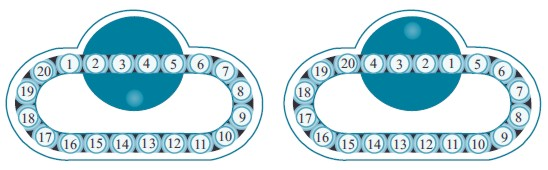
\includegraphics[width=0.5\textwidth]{notes/images/topspin.jpg}
    \caption{TopSpin}
    \label{fig:topspin}
\end{figure}

We can describe any move by saying what it does to the slots. For example, if you rotate the blue dial, that swaps the numbers in slots $1$ and $4$, as well as the numbers in slots $2$ and $3$. We would describe this as $(1 \ 4)(2 \ 3)$ in cycle notation. Rotating the entire thing clockwise can be described as $(1 \ 2 \ 3 \dots \ 20)$. Why is this a group?

\begin{itemize}
    \item Closure: If $M_1, M_2 \in T$, then $M_1 \circ M_2 \in T$ because $M_1 \circ M_2$ is a move.
    \item Identity: ``Do nothing" is the identity, $e \circ M = M \circ e = M$.
    \item Inverses: Every move can be undone.
    \item Associativity: Note that $T$ is a subset of $S_{20}$ (i.e. if $M_1, M_2, M_3 \in T$, then $M_1, M_2, M_3 \in S_{20}$). Since $S_{20}$ is a group, $M_1 \circ (M_2 \circ M_3) = (M_1 \circ M_2) \circ M_3$.
\end{itemize}

\end{example}

\subsection{The Subgroup Criterion}

\begin{proposition}[The Subgroup Criterion]
Let $(G, *)$ be a group. A nonempty subset $H$ of $G$ is a subgroup of $G$ iff, for every $a, b \in H$, we have $a * b^{-1} \in H$.
\end{proposition}

\begin{proof}
$(\implies)$. Apply the inverses property, so $b^{-1}$ is in $H$, and then apply closure, so $a * b^{-1}$ is in $H$. 

$(\impliedby)$. We want to show that $H$ is a group, so we show the four axioms:
\begin{itemize}
    \item Identity: Let $a \in H$ (which is possible since $H$ is nonempty). Then, $a * a^{-1} \in H$ by the hypothesis.
    \item Let $a \in H$. We just showed that $e \in H$, so $e * a^{-1} \in H$ by hypothesis.
    \item Closure: Let $a, b \in H$. We just showed that $b^{-1} \in H$, so $a * (b^{-1})^{-1} = a * b \in H$.
    \item Associativity is inherited from $G$.
\end{itemize}
\end{proof}

We can write a shorter proof that $T$ is a group by showing it is a subgroup of $S_{20}$ via the Subgroup Criterion (done in class, exercise for the reader).
\section{Lecture 9: 03/03/21}

\begin{example}
Last week we saw that $(\Z_4,+)$ and $U_5,\cdot_5$ have the same group table. Notice that we can pair up the elements quite nicely. This is like a bijection from $\Z_4$ to $U_5$ (or the other way around)!
\end{example}

\begin{question}
How can we define a general notion of two groups $(G,*)$ and $(H,\triangle)$ being the ``same'' in this way?
\end{question}
In general, we want some bijection $\varphi: G \rightarrow H$ such that 
\[\varphi(g_1*g_2) = \varphi(g_1) \triangle \varphi(g_2)\]

\subsection{Homomorphisms, Isomorphisms}

\begin{definition}[Homomorphism]
Let $(G,*)$ and $(H,\triangle)$ be two groups. Then a function $\varphi:G\rightarrow H$ is a \textit{homomorphism} if 
\[\varphi(g_1*g_2) = \varphi(g_1)\triangle \varphi(g_2)\]
for all $g_1,g_2\in G$.
\end{definition}
\begin{definition}[Isomorphism]
An \textit{isomorphism} is a bijective homomorphism. If there is an isomorphism from $G$ to $H$, we say that $G$ is \textit{isomorphic} to $H$, written $G \cong H$.
\end{definition}

\begin{example}
Are the following functions homomorphisms? Isomorphisms?
\begin{enumerate}
    \item $\varphi:\Z \rightarrow \Z_n$ given by $\varphi(k)=[k]_n$.
    \[\varphi(g_1+g_2) \stackrel{?}{=} \varphi(g_1) +_n \varphi(g_2)\]
    This is true because we know that 
    \[[g_1+g_2]_n = [g_1]_n +_n [g_2]_n\]
    So $\varphi$ is a homomorphism.
    \medskip
    
    Is $\varphi$ an isomorphism? \textbf{No.} $\varphi$ is not injective. We can see that $\varphi(0)=[0]_n=\varphi(n)$.
    \item $\varphi:\R_{>0} \rightarrow \R$ given by $\varphi(x)=\ln(x)$.
    The operation on $\R_{>0}$ is multiplication and the operation on $\R$ is addition, so we are really asking if
    \[\varphi(a\cdot b) \stackrel{?}{=} \varphi(a)+\varphi(b)\]
    \[\ln(a\cdot b) \stackrel{?}{=} \ln(a)+\ln(b)\]
    which is true! This is one of our logarithm rules.
    \medskip
    
    Is $\varphi$ an isomorphism? \textbf{Yes.} We can see graphically that $\varphi$ is surjective and injective, so $\varphi$ is an isomorphism. (We also know that $\varphi$ has an inverse, $\varphi^{-1}(x)=e^x$, so $\varphi$ is bijective.)
\end{enumerate}
\end{example}

\begin{note}
The ``number of elements in a group $G$'' (\textit{order} of $G$) is a structural property. If $G$ and $H$ are isomorphic, $|G|=|H|$.
\end{note}

\subsection{Kernel, Image}

\begin{definition}[Kernel]
Let $\varphi:G \rightarrow H$ be a homomorphism. The \textit{kernel} of $\varphi$, denoted $\ker\varphi$, is defined to be
\[\{g\in G | \varphi(g) = e_H\}\]
where $e_H$ is the identity of $H$.
\end{definition}

\begin{definition}[Image]
The \textit{image} of a homomorphism $\varphi:G \rightarrow H$ is the set
\[\im\varphi := \{\varphi(g) | g\in G\}\]
\end{definition}

\begin{note}
Some notation we use to say ``multiples of $n$'': $n\Z$
\end{note}


\section{Lecture 10: 03/08/21}

\subsection{Pigeonhole Principle}

\begin{definition}[Pigeonhole Principle]
If you put $n+1$ pigeons in $n$ holes, then there is a hole with more than $1$ pigeon.
\end{definition}

\begin{example}
Let $G$ be a finite group, and let $g\in G$. Prove that there exists a positive integer $n$ such that $g^n=e$.
\end{example}

\begin{proof}
Consider $g,g^2,g^3,\dots\in G$. Because we have an infinite list within a finite group, by the Pigeonhole Principle there exists $j, k \in \N$ with $j > k$ such that $g^j = g^k$. ``Multiplying'' both sides by $g^{-k}$ on the right, 
\[g^jg^{-k}=g^kg^{-k}\]
or \[g^{j-k}=e\]
\end{proof}

\subsection{Order}

\begin{definition}[Order]
Let $G$ be a group (finite or infinite), and let $g\in G$. If there exists $n\in \N$ such that $g^n=e$, the smallest such $n$ is called the \textit{order} of $g$. The order of $g$ is denoted by $|g|$ or $o(g)$.
\end{definition}

Recall that we once talked about the order of a \textit{group}, which was defined to be the number of elements in the group, also denoted by $|G|$. Now, however, we are talking about the order of an \textit{element} of a group.

\begin{example}
Find the order of $3$ in $U_{13}$.
\end{example}

\begin{proof}
Note that $3^1 = 3$, $3^2 = 9$, and $3^3 = 27$, but $[27]_{13} = [1]_{13}$, so the order is $3$.
\end{proof}

\begin{example}
Find the order of $5$ in $\Z_{20}$.
\end{example}

\textbf{Solution.} 
In $\Z_{20}$, the operation is addition, so raising $5$ to a power is like adding it to itself over and over. 
\[5=5\]
\[5+5=10\]
\[5+5+5=15\]
\[5+5+5+5=20=0\]
So the order of $5$ is $4$.

\begin{example}
Prove the following
\begin{proposition}
Let $G$ be a group. Suppose $a\in G$ has finite order. If $a^k=e$ for some $k\in \Z$, then $|a| \big| k$
\end{proposition}
\end{example}
\begin{proof}
Let $n=|a|$. (WTS: $n|k$.) By the division algorithm, there exists $q,r\in \Z$ such that $k=nq+r$ and $0\leq r<n$. (WTS: $r=0$.) Then, $r=k-nq$, and \[a^r=a^{k-nq}=a^ka^{-nq}=a^k(a^n)^{-q}\] by exponent rules. Then \[a^r=(a^n)^{-q}=e\] since $a^k=e$ and $n=|a|$, so $a^n=e$. 
\medskip

We've shown that $a^r=e$ and $r<n$, but $n$ is the smallest positive integer such that $a^n=e$ so $r$ must not be a positive integer. Since $r\geq 0$, the only possibility is that $r=0$.
\end{proof}

\subsection{Generators, Cyclic Groups}

\begin{definition}
Let $G$ be a group.
\begin{itemize}
    \item If $a\in G$, then the \textit{subgroup generated by $a$} is 
    \[\langle a \rangle := \{a^k|k\in \Z\}\]
    \item $G$ is \textit{cyclic} if $G=\langle a \rangle$ for some $a\in G$. We call $a$ the \textit{generator} of $G$.
\end{itemize}
\end{definition}

\begin{example}
Is $S_3$ cyclic? Why or why not?
\end{example}
\begin{proof}[Solution.] None of the below subgroups generated by elements of $S_3$ are equal to $S_3$:
\[\langle e \rangle = \{e\}\]
\[\langle (1\ 2) \rangle = \{(1\ 2), e\}\]
\[\langle (1\ 3) \rangle = \{(1\ 3), e\}\]
\[\langle (2\ 3) \rangle = \{(2\ 3), e\}\]
\[\langle (1\ 2\ 3) \rangle = \{(1\ 2\ 3), (1\ 3\ 2)e\}\]
\[\langle (1\ 3\ 2)\rangle = \{(1\ 2\ 3), (1\ 3\ 2)e\}\]
So $S_3$ is not cyclic.
\end{proof}

\begin{example}
If $G$ is a finite cyclic group with a generator $a$, how does $|G|$ relate to $|a|$?
\end{example}
\textbf{Solution.} We claim that $|a|=|G|$.
\begin{proof}[Sketch of the proof:]
Let $n=|a|$. 
\begin{itemize}
    \item Prove that $G=\{e,a,a^2,\dots,a^{n-1}\}$
    \begin{itemize}
        \item $\langle a \rangle \subseteq G$ by definition of $\langle a \rangle$
        \item $\langle a \rangle \supseteq G$: $G= \{a^k|k\in \Z\}$ so WTS: $a^k\in \{e,a,a^2,\dots,a^{n-1}\}$. Use the Division Algorithm to write $k=nq+r$. Show that $a^k=a^r$.
    \end{itemize}
    \item Prove that $e,a,a^2,\dots,a^{n-1}$ are distinct.
\end{itemize}
\end{proof}

\begin{example}
Prove or disprove: Every cyclic group is abelian.
\end{example}
\begin{proof}
Let $G$ be a cyclic group with a generator $a$. Let $x,y\in G$. Then $x =a^j$ and $y=a^k$ for some $j,k\in \Z$. Then $xy=a^ja^k=a^{j+k}$ and $yx=a^ka^j=a^{k+j}$, so $xy-yx$ since $j+k=k+j$.
\end{proof}
\section{Lecture 11: 03/10/21}

\begin{theorem}[Lagrange]
Let $G$ be a finite group. If $H$ is a subgroup of $G$, then $|H| \big| |G|$.
\end{theorem}

\subsection{Cosets!}

We will be using the tool of \textit{cosets}. If $G$ is a group (finite or infinite) and $H$ is a subgroup of $G$, and $g \in G$, then we define:

\begin{itemize}
    \item The \textit{left coset} is $gH = \{gh | h \in H\}$.
    \item The \textit{right coset} is $Hg = \{hg | h \in H\}$.
\end{itemize}

\begin{example}[$\Z_{12}$]
Consider the group $\Z_{12}$ and the subgroup $H = {0, 3, 6, 9}$. Then a non-repeating list of left cosets of $H$ in $\Z_{12}$ is:
\begin{itemize}
    \item $[0]_{12} + H = \{0, 3, 6, 9\}$
    \item $[1]_{12} + H = \{1, 4, 7, 10\}$
    \item $[2]_{12} + H = \{2, 5, 8, 11\}$
\end{itemize}

It turns out that the right cosets are exactly the same as these!
\end{example}

\begin{example}
Look back at the examples of cosets we have seen so far. What properties do you notice?
\begin{itemize}
    \item All cosets have the same number of elements, which is $|H|$.
    \item The sum of the number of elements in each distinct coset is $|G|$ because every element of $|G|$ is in exactly one coset.
\end{itemize}
Based on these properties, $|G|=(\mbox{\# of cosets})(\mbox{size of each coset})$
\end{example}

\begin{lemma}
Let $G$ be a finite group and $H$ be a subgroup of $G$. If $g\in G$, then $|gH|=|H|$.
\end{lemma}

\begin{proof}
(Strategy: find a bijection between $gH$ and $H$)\\
Let $f:H\rightarrow gH$ be defined by $f(h)=gh$. 
\begin{itemize}
    \item (injective) Suppose $f(h_1)=f(h_2)$ for some $h_1,h_2\in H$. By definition of $f$, 
    \[gh_1=gh_2\]
    By the left-cancellative property, $h_1=h_2$.
    \item (surjective) Let $b\in gH$. Then $b=gh$ for some $h\in H$. So $f(h)=gh=b$.
\end{itemize}
So $f$ is bijective, so $|H|=|gH|$.
\end{proof}

\subsection{Lagrange's Theorem!}

\begin{theorem}[Lagrange]
Let $G$ be a finite group. If $H$ is a subgroup of $G$, then $|H| \big| |G|$.
\end{theorem}

\begin{proof}[Proof of Lagrange's Theorem]
Let $G$ be a finite group and $H$ be a subgroup of $G$. Since every element of $G$ is in exactly one left coset, 
\[|G| = (\mbox{\# of left cosets})(\mbox{size of each left coset})\]
\[|G| = (\mbox{\# of left cosets})|H|\]
by our lemma. So $|H|\big| |G|$ (and the number of left cosets is $\frac{|G|}{|H|}$.
\end{proof}

\begin{corollary}
Let $|G|$ be a finite group and $g\in G$. Then $|g|\,\big|\,|G|$.
\end{corollary}
\begin{proof}
By Lagrange's Theorem, $|\langle g \rangle\| \,\big| \,|G|$. Last time we showed that $|g| = |\langle g\rangle|$. So $|g| \,\big| \,|G|$.
\end{proof}

\begin{corollary}
Let $G$ be a finite group with prime order. Then $G$ is cyclic, and any non-identity element is a generator for $G$.
\end{corollary}

\begin{proof}
Let $|G|$ be a finite group with prime order. Let $g$ be any non-identity element of $G$. (WTS: $\langle g \rangle =G $). Since $|g| \,\big| \,|G|$ and $|G|$ is prime, either $|g|=1$ or $|g|=|G|$. Since $g\neq e$, $|g|\neq 1$ so $|g|=|G|$. So, $\langle g \rangle$ has $|G|$ elements, so $\langle g \rangle $=G .
\end{proof}
\section{Lecture 12: 03/15/21}

\subsection{Operation on Cosets, Normal Subgroups}

Let $H$ be a subgroup of $G$.

\begin{lemma}
Let $g_1, g_2 \in G$. Then $g_1H = g_2H$ iff $g_1 \in g_2H$. This means that $g_1 = g_2 h$ for some $h \in H$.
\end{lemma}

\begin{definition}
We defined $*_l$ on $\{\text{left cosets of $H$ in $G$}\}$ by:
\begin{align*}
    (aH) *_l (bH) := abH.
\end{align*}
\end{definition}

When is $*_l$ well-defined?\\

We want it to be the case that if $a_1H = a_2H$ an $b_1H = b_2H$, then $a_1b_1H = a_2b_2H$.

We know that $a_1 = a_2h_1$ and $b_1 = b_2h_2$ for some $h_1, h_2 \in H$. We want to show that $a_1b_1 = a_2b_2h_3$ for some $h_3 \in H$.

Thus, our expression that we want to show is equivalent to:
\begin{align*}
    a_1b_1 &= a_2b_2h_3 \\
    \iff (a_2h_1)(b_2h_2) &= a_2b_2h_3 \\
    \iff b_2^{-1}h_1b_2h_2 &= h_3
\end{align*}

Thus, we need $b_2^{-1}h_1b_2$ to be in $H$. We write $g = b_2^{-1}$ and $h = h_1$, so that we now need $ghg^{-1} \in H$ for all $g \in G$ and $h \in H$, which is equivalent to $H$ being a normal subgroup of $G$ (denoted $H \triangleleft G$).

\subsection{Quotient Groups}

\begin{proposition}
Suppose that $H \triangleleft G$. We write $G/H$ for the set of left cosets of $H$ in $G$. We've defined an operation on $G/H$ by $(aH)(bH) := abH$, and we've seen that this operation is well-defined. Prove that $G/H$ is a group under this operation.\\

We read $G/H$ as ``$G$ mod $H$" and call it a \textbf{quotient group} or \textit{factor group}.
\end{proposition}

We can check the axioms as follows:
\begin{itemize}
    \item Closure: If $aH, bH \in G/H$, then $(aH)(bH) = abH$ is a left coset, so $abH \in G/H$.
    \item Associativity: Let $aH$, $bH$, $cH$ be in $G/H$. Then $((aH)(bH)(cH) = ((ab)cH) = (a(bc)H) = (aH)((bH)(cH))$ (by associativity in $G$).
    \item Identity: Let $e$ be the identity of $G$. Then $(aH)(eH) = (eH)(aH) = aH$.
    \item Inverses: Let $g \in G$. Then $g^{-1}H$ is the inverse of $gH$ since $(g^{-1}H)(gH) = (gH)(g^{-1}H) = eH$.
\end{itemize}

\begin{example}
Let $G$ be any group. We examine edge cases. We can show that $G$ and $\{e\}$ are normal subgroups of $G$.

\begin{itemize}
    \item Describe the quotient group $G/G$.
    \begin{align*}
        G/G &= \{\text{left cosets of $G$ in $G$}\} \\
        &= \{eG\}.
    \end{align*}
    so this quotient group has just one element!
    \item Describe the quotient group $G/\{e\}$.
    \begin{align*}
        G/\{e\} &= \{\text{left cosets of $\{e\}$ in $G$}\} \\
        &= \{\{g\} \ \forall g \in G\}
    \end{align*}
    so $|G/\{e\}| = |G|$.
\end{itemize}
\end{example}

\begin{example}
Explain why $\Z \triangleleft \R$, and describe the quotient group $\R / \Z$.
\end{example}

\begin{proof}
Two different ways to show that $\Z$ is a normal subgroup of $\R$:
\begin{itemize}
    \item $\R$ is abelian
    \item If $g \in \R$ and $h \in \Z$, then $g + h + (-g) = h \in \Z$.
\end{itemize}
The left cosets are $a + \Z$, so we have:
\[
\R/\Z = \{a + \Z | 0 \le a < 1\}
\]
\end{proof}

\begin{example}
Prove that, if $H \triangleleft G$ and $a \in G$, then $aH = Ha$.
\end{example}

\begin{proof}
Suppose $H \triangleleft G$ and $a \in G$. Then we show both sides:
\begin{itemize}
    \item $\subseteq$. Let $x \in aH$. Then $x = ah$ for some $h \in H$. We can rewrite $x = aha^{-1}a$. Since $H$ is a normal subgroup of $G$, $aha^{-1} \in H$, so $x \in Ha$.
    \item $\supseteq$. Let $x \in Ha$. Then $x = ha$ for some $h \in H$. We can rewrite $x = aa^{-1}ha$, and $a^{-1}ha \in H$, so $x \in aH$.
\end{itemize}
\end{proof}
\section{Lecture 13: 03/17/21}

Recall from last time:
\begin{itemize}
    \item If $H \triangleleft G$, $G/H = \{\text{cosets of $H$ in $G$}\}$ is a group with operation $(aH)(bH) = abH$.
    \item Examples:
    \begin{itemize}
        \item $\Z/n\Z = \Z_n$. E.g. $\Z/4\Z = \{0 + 4\Z, 1 + 4 \Z, 2 + 4\Z, 3 + 4\Z\}$.
        \item If $G$ is a group, then $G/G$ is the trivial group, and $G/\{e\} \cong G$.
    \end{itemize}
\end{itemize}

\subsection{First Isomorphism Theorem}

\begin{theorem}[First Isomorphism Theorem]
For a group $G$ and a homomorphism $\varphi: G \to H$, we have that:
\[
G/\ker (\varphi) \cong \im \varphi.
\]
\end{theorem}

We give examples of this:

\begin{example}
If $\phi: G \to H$ is a group homomorphism with $\ker \phi = \{e_G\}$, we have seen previously in Problem Set 7 that $G \cong \im \phi$. Then $G/\ker\phi = G /\{e_G\} \cong \im \phi$.
\end{example}

\begin{example}
Let $n \in \N$, and let $\phi : \Z \to \Z_n$ be defined by $\phi(x) = [x]_n$. Then $\ker \phi = n\Z$, and $\Z/\ker\phi = \Z/n\Z = \Z_n$, and $\im \phi = \Z_n$, so $\Z/\ker\phi \cong \im \phi$.
\end{example}

\begin{example}
Consider the homomorphism $\phi : \Z \to \R^\times$ defined by $\phi (n) = (-1)^n$. Then $\ker \phi = \{n | (-1)^n = 1\} = 2\Z$, $\Z/\ker\phi = \Z/2\Z = \Z_2$, and $\im \phi = \{(-1)^n | n \in \Z\} = \{\pm 1\}$. Since there is only one group of order $2$ (previous homework), these groups must be isomorphic.
\end{example}

Now we give a proof of the First Isomorphism Theorem:

\begin{proof}
\begin{enumerate}
    \item First we must prove the kernel is a normal subgroup so that the quotient is well-defined (i.e. $\ker \phi \triangleleft G$). This is proved in Problem Set 7 $\# 2(e)$.
    \item $G /\ker \phi \cong \im \phi$. We will define $\psi : G /\ker \phi \to \im \phi$ by $\psi (gK) = \phi(g)$. We want to show that $\psi$ is a bijection, a homomorphism, and well-defined.
\end{enumerate}

Let $K = \ker \phi$. Define $\psi : G/K \to \im \phi$ by $\psi(gK) = \phi(g)$. To show it is well-defined, suppose $g_1K = g_2K$ for some $g_1, g_2 \in G$. Then $g_1 \in g_2K$, so we can write $g_1 = g_2k$ for some $k \in K$. Then $\phi(g_1) = \phi(g_2k) = \phi(g_2)\phi(k) = \phi(g_2)$ since $k \in \ker\phi$. This means that $\psi(g_1K) = \psi(g_2K)$, so $\psi$ is well defined (equal things map to the same thing). \\

Now to show $\psi$ is a homomorphism, let $g_1K, g_2K \in G/K$. Then,
\begin{align*}
    \psi((g_1K)(g_2K)) &= \psi(g_1g_2K) \\
    &= \phi(g_1g_2) \\
    &= \phi(g_1)\phi(g_2) \\
    &= \psi(g_1K)\psi(g_2K)
\end{align*}
which means that $\psi$ is a homomorphism.\\

Now to show that $\psi$ is a bijection, we show it is injective and surjective. For injectivity, suppose that $\psi (g_1K) = \psi(g_2K)$ for some $g_1K, g_2K \in G/K$. Then by definition of $\psi$, $\phi(g_1) = \phi(g_2)$. By Problem set $7$ $\# 2(f)$, we have $g_1 = g_2k$ for some $k \in \ker \phi$, so $g_1 \in g_2K$, so $g_1K = g_2K$.\\

For surjectivity, let $h = \im \phi$. Then $\exists g \in G$ such that $\phi(g) = h$. This means that $\psi(gK) = \phi(g) = h$, so $\psi$ is surjective (and injective) and thus bijective.
\end{proof}
\section{Lecture 14: 03/22/21}

Today we will be talking about cardinality of infinite sets like $\N$, $\Z$, $\Q$, and $\R$. Note that today's proofs are surprising! They will probably feel unintuitive and the kinds of things that mathematicians thought about for years so don't feel discouraged! 

\subsection{Cardinality (Infinite Sets!)}

\begin{definition}
Let $A$ and $B$ be sets. We say that $A$ \textit{has the same cardinality} as $B$, written $|A|=|B|$, if there's a bijection $f:A\rightarrow B$.
\end{definition}

\begin{example}
We know for example that $|\Z| = |3\Z|$ namely that there is a bijection between the two sets. There is another intuition here that has to do with the  density of the sets. We will not cover this today but you can look at it if you are curious!
\end{example}

Recalling a proof from Problem Set 4, we proved that the function $g: \Z \to \N$ given by 
\[
g(k) = \begin{cases}
        2k+1 \text{ if $k > 0$,}
        \\
        -2k \text{ if $k < 0$}
        \end{cases}
        is a bijection. 
\]

\subsection{Countable Sets}

\begin{definition}
A set $S$ is \emph{countably infinite} if $|S| = |N|$. Different sources use the word countable diferently: soem use it to mean ``countably infinite", while others use it to mean ``finite or countably infinite". 
\end{definition}

\begin{example}
Perhaps surprisingly, $\Z \times \Z$ is countable. Can you give a picture proof of this?
\begin{center}
    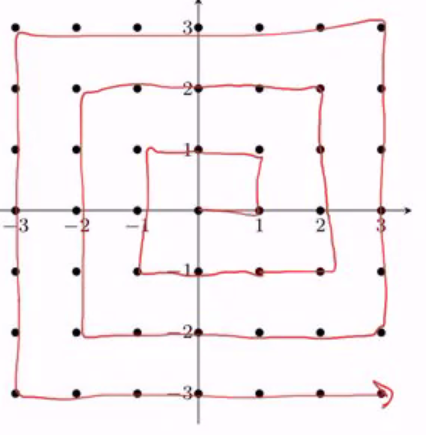
\includegraphics[scale=.25]{notes/images/picture_proof.PNG}
\end{center}
\end{example}

\begin{example}
Is $\Q$ countable or uncountable? To develop our intuition for this, let's think about the fact that we can represent a rational number as $\frac{a}{b}$ where $b \neq 0$. Now if we define our bijection as $\frac{a}{b} \to (a, b)$. We can then ignore the lower two quadrants as they are the same as other points. And then we can use a similar spiral as our previous proof to pictorially develop a bijection. We can now say that $\N, \Z, \Z \times \Z, \Q$ are all countable (all have the same cardinality. 
\end{example}

At this point you may be wondering, is everything countable? Let's look at an answer to that question. 

\begin{example}
\begin{claim}
The open interval $(0, 1)$ is uncountable. 
\end{claim}
\begin{proof}
This is often referred to as Cantor's diagonal proof (diagonalization). Let $f: \N \to (0, 1)$. We'll show that $f$ isn't surjective. Write $f(1), f(2), f(3), \dots$ as decimals not ending in repeating $9$s (think about what $\bar{.9}$ is). We can consider one such an example:
\begin{align*}
    f(1) &= .7654157\dots \\
    f(2) &= 0.1543296 \dots \\
    f(3) &= 0.5000000 \dots 
\end{align*}
We now want to construct an example that doesn't get hit by our function. Let's call this number $w$. Let $w$ be the decimal whose $n$-th digit is 
\[
\text{digit = } \begin{cases}
        5 \text{ if the $n$-th digit of $f(n)$ isn't $5$,}
        \\
        6 \text{ if otherwise.}
        \end{cases}
\]
We can start constructing our $w$ using our previous examples. We would get something like $w = 0.565 \dots$. We have that $w \in (0,1)$, but could it be equal to $f(1)$? No, because we changed a digit. This is true for all $n$ i.e. $\forall n \in \N \; w \neq f(n)$ as it has a different $n$-th digit. So, $f$ isn't surjective!
\end{proof}
\end{example}

\begin{example}
There's a precise way to measure the length of a subset of $\R$; we won't go into all of the details (this is a field of math known as measure theory), but here are some basic facts:
\begin{enumerate}
    \item The length of any subset of $\R$ is $\geq 0$.
    \item The length of an open interval $(a, b)$ is $b-a$.
    \item If $A \subseteq B$, then (length of $A$) $\leq$ (length of $B$).
    \item The length of $A \cup B$ is $\leq$ to $length(A) + length(B)$.
\end{enumerate}
Let $S$ be a countably infinite subset of $R$. What can you say about the length of $S$? Letting $S$ be such a subset of $R$. Then, there's a bijection $f: \N \to S$. Let $\epsilon > 0$. Thinking about the intervals around $f(n)$ for $n \in \N$ as being progressively tighter around $f(n)$. Let:
\begin{align*}
    I_1 &= (f(1) - \frac \epsilon 4, f(1) + \frac \epsilon 4 \\
    I_2 &= (f(2) - \frac \epsilon 8, f(2) + \frac \epsilon 8 \\
    I_3 &= (f(3) - \frac \epsilon {16}, f(3) + \frac \epsilon {16} \\
\end{align*}

Let $I = I_1 \cup I_2 \cup I_3 \cup \dots$. Then $S \subseteq I$, so $length(s) \leq length(I) \leq length(I_1) + length(I_2) + \dots$. This is equal to $\frac{\epsilon}{2} + \frac{\epsilon}{4} + \frac{\epsilon}{4} + \frac{\epsilon}{8} + \dots = \epsilon$. We have shown that the $length(s) \leq \epsilon$ for every $\epsilon > 0$, so the length of $S$ must be $0$!



We can provide another proof of this in the following way:
\begin{proof}
$(0,1)$ has length $1$, but countable subsets of $R$ have length $0$.
\end{proof}
\end{example}

\begin{example}
Let $a,b \in \R$ with $a<b$. True or false:
\begin{enumerate}
    \item There is a rational number $q$ with $a < q < b$.
    This is true. For a proof, refer to worksheet 15!
    \item There is an irrational number $r$ with $a < r < b$. 
    We can make a straightforward argument to show that this is true. Consider the fact that the length of the interval $(a,b)$ is greater than $0$. Additionally, the length of the rationals is $0$. Therefore, there must be irrational numbers in $(a, b)$.
\end{enumerate}
\end{example}

To take stock of what we saw today, we have that $\N, \Z, \Q$ all have the same cardinality and are namely countable. We saw that $(0,1)$/any open interval and $\R$ are uncountable and have the same cardinality. We will leave you with an interesting question called the Continuum hypothesis: is there a cardinality in between the integers and the reals? It has been shown to be both consistent and inconsistent i.e. unprovable. There is a continuing debate about it to this day. 

\section{Lecture 15: 03/24/21}

\subsection{Dihedral Group}

Today will mostly be exam review, but before this, let's introduce a new group! This will be the symmetries of a square. 
\smallbreak
To think about this, let's consider a square cushion. We can do a couple things with this (besides sitting on it). The first thing we can do is consider rotating the cushion. If we label the corners, we see that we can see these moves as permutations of the corners. We call this group $D_4$ which is the symmetries of a square and a subgroup of $S_4$.\\

(See \href{https://canvas.harvard.edu/courses/79110/files/12034681}{Worksheet 16} for Midterm Exam Review problems)
\section{Lecture 16: 03/29/21}

\begin{example}[Triangle Inequality]
If $|a - 3| < 0.1$ and $|b - 4| < 0.2$, then $|a + b - 7| < 0.3$.
\end{example}

\begin{proof}
We can show this using the triangle inequality:
\begin{align*}
    |(a - 3) + (b - 4)| \le |a - 3| + | b - 4| < 0.1 + 0.2 = 0.3.
\end{align*}
\end{proof}

\subsection{Axioms for $\R$}

\begin{definition}[Axioms for $\R$] 
\quad
\begin{enumerate}
    \item $(\R, +)$ is an abelian group with identity element $0$.
    \item $(\R \backslash \{0\}, \cdot)$ is an abelian group with identity element $1$.
    \item $x(y + z) = xy + xz$ for all $x, y, z \in \R$.
    \item There is a relation $<$ on $\R$ satisfying the following properties:
    \begin{enumerate}
        \item If $x, y \in \R$, exactly one of the following is true: $x<y$, $y < x$, or $x = y$.
        \item If $x<y$ and $y < z$, then $x < z$.
        \item If $x < y$, then $x + z < y + z$.
        \item If $x > 0$ and $y > 0$, then $xy > 0$.
    \end{enumerate}
    \item The limit of a sequence for $\pi$ converges.
\end{enumerate}
\end{definition}

\subsection{Sequences, Convergence}

\begin{definition}[Sequences]
A \textit{sequence} is an infinite ordered list of numbers.
\end{definition}
Notations:
\begin{itemize}
    \item $(1,2,4,8,\dots)$
    \item $(2^n)^\infty_{n=0}$
\end{itemize}

\begin{example}
\label{ex:real-analysis-1}
$\lim_{n\to \infty}6+\frac{6\sin(n)}{n}=6$
\end{example}

\begin{definition}[Sequence Convergence]
A sequence $(a_n)$ \textit{converges} to a limit $L$ if, for every $\varepsilon>0$, there exists $N$ such that for all $n \in N$ with $n > N$, $|a_n - L| < \varepsilon$.
\end{definition}
\begin{note} Structure of a proof that $(a_n) \rightarrow L$:
\begin{itemize}
    \item Let $\varepsilon >0$.
    \item Let $N=$ something you came up with depending on $\varepsilon$
    \item Let $n>N$
    \item Show that $|a_n-L|<\varepsilon$
\end{itemize}
\end{note}

We will now prove Example \ref{ex:real-analysis-1}.

\begin{proof}
Let $\varepsilon > 0$. 
\newline
{
\color{blue}
Scratch work: We want $|6+\frac{4\sin(n)}{n}-6|<\varepsilon
$ when $n>N$. So, we want $\frac{4\sin(n)}{n}<\varepsilon$. We know that
\[
\frac{4}{n} |\sin n | \le \frac 4 n < \frac 4 N.
\]
We want $\frac 4 N \le \varepsilon$, so we can let $N \ge \frac 4 \varepsilon$.
}
\\

Let $N = \frac 4 \varepsilon$. Let $n > N$. Then:
\begin{align*}
    | 6 + \frac{4\sin n}{n} - 6 | &= \frac{4}{n}|\sin n| \\
    &\le \frac 4 n \quad \text{since }|\sin n| \le 1 \\
    &< \frac 4 N \quad \text{since } n > N \\
    &=\varepsilon \quad \text{since }N = \frac 4 \varepsilon.
\end{align*}
\end{proof}

\begin{example}
Prove that $\lim_{k \to \infty} \frac{3k-2}{5k} = \frac 3 5$.
\end{example}

\begin{proof}
Let $\varepsilon > 0$. Let $N = \frac 2 {5\varepsilon}$. Let $k > N$. Then,
\begin{align*}
    \left|\frac{3k-2}{5k} - \frac 3 5 \right| &= \left|\frac 3 5 - \frac 2 {5k} - \frac 3 5\right| \\
    &= \frac{2}{5k} \\
    &< \frac{2}{5N} \\
    &= \varepsilon.
\end{align*}
\end{proof}

\subsection{Divergence}

\begin{example}
The sequence $(1, -1, 1, -1, 1, -1, \dots)$ diverges.
\end{example}

\begin{definition}[Divergence]
A sequence $(a_n)$ diverges if $(a_n) \nrightarrow L $  for any $L \in \R$.
\end{definition}

To prove something diverges, let $L \in \R$, and we prove that $(a_n) \nrightarrow L$ (show that there exists $\varepsilon$ that doesn't work. Next time we'll show an easier way to prove some sequences diverge.

\subsection{Theorems on Convergence}

\begin{theorem}[Algebraic Limit Theorem]
Let $(a_n)$ and $(b_n)$ be convergent sequences, and let $a = \lim_{n \to \infty} a_n$ and $b = \lim_{n \to \infty} b_n$.
\begin{enumerate}
    \item $(ca_n) \to ca$ for all $c \in \R$.
    \item $(a_n+b_n) \to a+b$  
    \item $(a_nb_n) \to ab$.
    \item If $b_n \neq 0$ for all $N \in \N$, and if $b \neq 0$, then $\left(\frac{a_n}{b_n}\right) \to \frac a b$.
\end{enumerate}
\end{theorem}

\begin{theorem}[Order Limit Theorem]
If $a_n \leq b_n$ for all $n\in \N$, then $a\leq b$.
\end{theorem}

We will prove part $(2)$ of the Algebraic Limit Theorem. We have that:

\begin{proof}
Let $\varepsilon > 0$. Since $(a_n) \to a$, there exists $N_1$ such that, if $n > N_1$, then $|a_n - a| < \varepsilon /2$. And since $(b_n) \to b$, there exists $N_2$ such that, if $n > N_2$, then $|b_n - b| < \varepsilon /2$. Let $N=max(N_1,N_2)$. Let $n>N$. Then $n>N_1$ and $n>N_2$, so $|a_n-a|<\frac{\varepsilon}{2}$ and $|b_n-b|<\frac{\varepsilon}{2}$.
Then,
\begin{align*}
    |a_n + b_n - (a+b)| &\le |a_n - a| + |b_n - b| \\
    &< \frac \varepsilon 2 + \frac \varepsilon 2 \\
    &= \varepsilon.
\end{align*}
\end{proof}

We will prove the Order Limit Theorem:
\begin{proof}(by contrapositive)
Suppose $a>b$. Let $\varepsilon = \frac{a-b}{2}$. Since $(a_n)\to a$, there exists $N_1$ such that if $n>N_1$, then $|a_n-a|<\varepsilon$. And, since $(b_n)\to b$, there exists $N_2$ such that if $n>N_2$, then $|b_n-b|<\varepsilon$. Let $n > \max(N_1, N_2)$. Then $|a_n - a| < \varepsilon$ and $|b_n - b| < \varepsilon$, Then $a_n > a - \varepsilon = \frac{a+b}2$ and $b_n < b + \varepsilon = \frac{a+b}2$. So, $a_n > b_n$.
\end{proof}
\section{Lecture 17: 04/05/21}

Recall:
\begin{itemize}
    \item A sequence $(a_n)$ in $\R$ converges to a limit $L$ if, for every $\varepsilon > 0$, there exists $N$ such that, for all $n > N$, $|a_n - L| < \epsilon$.
\end{itemize}

\subsection{Monotonic Sequence Property}

\begin{theorem}[Monotonic Sequence Property]
If $(a_n)$ is an increasing sequence which is bounded above, then $(a_n)$ converges (to a limit in $\R$).
\end{theorem}

We have an immediate corollary of this property:
\begin{corollary}
If $(a_n)$ is a decreasing sequence which is bounded below, then $(a_n)$ converges.
\end{corollary}

\begin{proof}
Let $(a_n)$ be a decreasing sequence bounded below by $M$. Then $(-a_n)$ is an increasing sequence bounded above by $-M$, so $(-a_n)$ converges by the Monotonic Sequence Property. Then $(a_n)$ converges by the Algebraic Limit Theorem.
\end{proof}

\subsection{Boundedness}

\begin{definition}[Boundedness]
A set or sequence in $\R$ is \textit{bounded} if there exists $M$ such that $|x| \le M$ for all $x$ in the set or sequence. (This is equivalent to being both bounded above and bounded below).
\end{definition}

\begin{example}
Prove every convergent sequence is bounded.
\end{example}
\begin{proof}
Let $(a_n)_{n=1}^\infty$ be a convergent sequence and $L = \lim_{n=1}^\infty a_n$. Since $1>0$, there exists $N\in \N$ such that, for all $n>N$, $|a_n-L|<1$. Let $M=max(|a_1|,|a_2|,\dots,|a_N|, 1+|L|)$. Let $n\in N$. 
\begin{itemize}
    \item If $n\leq N$, then $|a_n| \leq M$ by definition of $M$.
    \item If $n>M$, then $|a_n-L|<1$, so
    \begin{align*}
        |a_n| &= |a_n-L+L|\\
        &\leq |a_n-L|+|L| \quad\quad \text{by the triangle inequality}\\
        &< 1+|L|\\
        &\leq M
    \end{align*}
\end{itemize}
So, $|a_n| \leq M$.
\end{proof}

\begin{definition}[Subsequence]
Let $(a_n)$ be a sequence. If $n_1 < n_2 < n_3 < \dots$, then $(a_{n_1}, a_{n_2}, a_{n_3}, \dots)$ is a \textit{subsequence} of $(a_n)$.
\end{definition}

\begin{proposition}
If a sequence $(a_n)$ converges to some limit $L$, then every subsequence also converges to $L$.
\end{proposition}

\begin{theorem}[Bolzano-Weierstrass]
Every bounded sequence has a convergent subsequence.
\end{theorem}
\section{Lecture 18: 04/07/21}

Today we will be looking at the Bolzano-Weierstrass Theorem. We will also cover sequences in $\R^m$. This theorem is the longest, most involved theorem we will prove in Math 101, so don't be worried if it takes a couple of going's over for it to click!.

\subsection{Bolzano-Weierstrass}

\begin{theorem}[Bolzano-Weierstrass Theorem]
Every bounded sequence has a convergent subsequence.
\end{theorem}

\begin{proof}
Let $(x_n)^\infty_{n=1}$ be a bounded sequence. Then, there exists $M\in \R$ such that $|x_n| \leq M$ for all $n$. \footnote{Note: for any CS-minded readers, the way that we go about this proof is very similar to a binary search algorithm}\\

\emph{Our overall strategy here is that we want to leverage the squeeze theorem to show that $(a_k)$ and $(b_l)$ converge to same limit, then squeeze theorem says that $x_{n_k}$ converges to that limit too.} \\

Let $a_1 = M$ and $b_1 = M$. Bisect $[a_1, b_1]$ into $2$ closed subintervals. At least one of the subintervals has infinitely many terms of $(x_n)$, so let $[a_2, b_2]$ be such a subinterval. \\

Bisect $[a_2, b_2]$, $[a_3, b_3]$ and continue this process. Since $[a_1, b_1] \supseteq [a_2, b_2] \supseteq [a_3, b_3] \supseteq \dots$, $a_1 \le a_2 \le a_3 \le \dots$. So, $(a_k)$, is increasing. Also, $(a_k)$ is bounded above by $b_1$, so $(a_k)$ must converge by the MSP. Let $L = \lim_{k\to\infty}a_k$. \\

The length of $[a_k, b_k]$ is $b_k - a_k = \frac{4M}{2^k}$ by construction, so $\lim_{k\to\infty}(b_k-a_k) = 0$.  Since $b_k = (b_k -a_k) + a_k$, $\lim_{k\to\infty}b_k = 0 + L = L$ by the Algebraic Limit Theorem.\\

Now, we'll construct a convergent subsequence $(x_{n_k})$ of $(x_n)$ as follows:
\begin{enumerate}
    \item The first term we said doesn't really matter, so we simply say: Let $n_1 \in \N$.
    \item Since $[a_2, b_2]$ has infinitely many terms of $(x_n)$, there exists $n_2 > n_1$, such that $x_{n_2} \in [a_2, b_2]$.
    \item  Since $[a_3, b_3]$ has infinitely many terms of $(x_n)$, there exists $n_3 > n_2$, such that $x_{n_3} \in [a_3, b_3]$.
    \item $\dots$
\end{enumerate}
Since $x_{n_k} \in [a_k, b_k]$, we have $a_k \leq x_{n_k} \leq b_k$. Since $\lim_{k\to\infty} a_k = \lim_{k\to\infty}b_k = L$, $\lim_{k\to\infty}x_{n_k} = L$ by the Squeeze Theorem.
\end{proof}

Now let's move to considering sequences in $\R^m$. A small notational note is that when we want to talk about a point we denote this with an arrow i.e. $\vec{x}$. \\

Let's start with a familiar definition in $\R$. \begin{definition}
A sequence $(x_n)$ in $\R$ converges to a limit $L$ if, for every $\varepsilon > 0$, there exists $N$ such that, for all $n > N$, $|x_n - L| < \varepsilon$. 
\end{definition}
To generalize this to $\R^m$, consider
\begin{definition}
A sequence $(\vec{x}_n)$ in $\R^m$ converges to a limit $\vec{L}$ if, for every $\varepsilon > 0$, there exists $N$ such that, for all $n > N$, $||\vec{x_n} - \vec{L}|| < \varepsilon$.
\end{definition}
Some notes on notation:
\begin{itemize}
    \item In $\R$, $|a|$ is the distance between $a$ and $0$.
    \item in $\R^m$, distance between $\vec{a} = (a_1, \dots, a_m)$ and $\vec{0} = (0, \dots, 0)$ is $||\vec{a}|| = \sqrt{a_1^2 + \dots + a_m^2}$. This is referred to as the norm of a. 
\end{itemize}
Some facts about $\R^m$:
\begin{itemize}
    \item The triangle inequality still holds, namely that $||\vec{x} + \vec{y}|| \le ||\vec{x}|| + ||\vec{y}||$.
    \item A set/sequence in $\R^m$ is bounded if there exists $M \in \R$ such that $||\vec{x}|| \leq M$ for all $\vec{x}$ in the set/sequence.
\end{itemize}
\section{Lecture 19: 04/12/21}

\subsection{Function Continuity}

\begin{definition}[Function Continuity]\
\quad
\begin{enumerate}
    \item Calculus $1$ definition: $f$ is continuous at $c$ if $\lim_{x \to c} f(x) = f(c)$.
    \item Actual definition: Let $f: \R^m \to \R^n$ and $\vec c \in \R^m$. We say $f$ is \textit{continuous} at $\vec c$ if for every $\varepsilon>0$, there exists a $\delta>0$ such that, for every $\vec{x}\in \R^m$ such that $|\vec{x}-\vec{c}| <\delta$, we have $||f(\vec x) - f(\vec c)|| < \varepsilon$.
\end{enumerate}
\end{definition}

\begin{example}
Suppose you want to prove a function $f: \R^m \to \R^n$ is continuous at $\vec c$. The general structure of the proof should go as follows:
\begin{enumerate}
    \item Let $\varepsilon > 0$.
    \item Let $\delta$ be something you come up with based on $\varepsilon$.
    \item Let $\vec x \in \R^m$ such that $||\vec x - \vec c|| < \delta$. 
    \item $\vdots$ (do some things)
    \item Therefore, $||f(\vec x) - f(\vec c) || < c$.
\end{enumerate}
\end{example}

\begin{example}
Prove that $f : \R \to \R$ given by $f(x) = 2x + 1$ is continuous at $3$.
\end{example}

\textcolor{blue}{
Scratchwork: want:
\begin{align*}
    |f(x) - f(3)| &< \varepsilon \qquad \text{when } |x - 3| < \delta \\
    |2x+1 - 7| &< \varepsilon \\
    |2x - 6| &< \varepsilon \\
    2|x - 3| &< \varepsilon \\
    \implies \text{we want}\quad 2\delta &\le \varepsilon.
\end{align*}
Let $\delta = \frac \varepsilon 2$.
}

\begin{proof}
Let $\delta = \frac \varepsilon 2$. Let $x \in \R$ such that $|x - 3| < \delta$. Then,
\begin{align*}
    |f(x) - f(3)| &= |2x + 1 - 7| \\
    &= |2x - 6| \\
    &= 2|x-3| \\
    &< 2\delta \\
    &= \varepsilon \qquad \text{since }\delta = \frac \varepsilon 2.
\end{align*}
\end{proof}

\begin{example}
Prove that $f: \R \to \R$ given by $f(x) = x^2$ is continuous at $5$.
\end{example}

\textcolor{blue}{
Scratchwork: want
\begin{align*}
    |f(x) - f(5)| &< \varepsilon \quad \text{when } |x - 5| < \delta . \\
    |x^2 - 25| &< \varepsilon \\
    |x-5||x+5| &< \varepsilon \\
\end{align*}
Let's decide $\delta \le 1$. Then $|x - 5| < 1$. We have $4 < x < 6$, so by the triangle inequality 
\[
|x + 5| \le |x| + 5 < 6 + 5 = 11.
\]
Thus, if $|x - 5| < \delta$, then $|x - 5||x+5| < \delta \cdot 11$, so we also want $\delta \le \frac{\varepsilon}{11}$.
}
\begin{proof}
Let $\varepsilon > 0$. Then $\delta = \min\left(1, \frac \varepsilon, 11\right)$. Let $x \in \R$ such that $|x - 5| < \delta$. Then,
\begin{align*}
    |f(x) - f(5)| = |x^2 - 25| = |x-5||x+5| \qquad \qquad  (*)
\end{align*}
Let's first bound $|x+5|$. Since $|x-5| < \delta \le 1$, $4 < x < 6$, so
\begin{align*}
    |x+5| &\le |x| + |5| \qquad \text{by triangle inequality}\\
    &< 6+5.
\end{align*}
Going back to $(*)$, 
\begin{align*}
    |f(x) - f(5)| &= |x-5||x+5| \\
    &< \delta \cdot 11 \\
    &\le \varepsilon \qquad \text{since }\delta \le \frac{\varepsilon}{11}.
\end{align*}
\end{proof}

\begin{example}
Prove that $f : \R \to \R$ given by $f(x) = x^3$ is continuous at $-3$. (Hint: $x^3 + 27 = (x+3)(x^2 - 3x+9)$.
\end{example}

\textcolor{blue}{
Scratchwork:
want $|f(x) - f(-3) = |x+3||x^2 - 3x+9| < \varepsilon$ when $|x+3 < \delta$. If we make $\delta \le 1$, then $|x+3| < 1$, so $-4 < x < -2$. Then $|x^2 - 3x + 9| \le |x|^2 + 3|x| + 9 < 4^2 + 3(4) + 9 = 37$.\\
}

In the actual proof, we start with: let $\varepsilon > 0$. Let $\delta = \min\left(1, \frac \varepsilon {37}\right)$.

\begin{example}
Let $f, g: \R^m \to \R^n$. Prove that, if $f$ and $g$ are both continuous at some point $\vec c \in \R^m$, then so is $f - 2g$.
\end{example}

\textcolor{blue}{
Scratchwork: Want $||(f-2g) (\vec x) - (f - 2g) ( \vec c)|| < \epsilon$ when $||\vec x - \vec c|| < \delta$. This is equivalent to:
\begin{align*}
    ||f(\vec x) - f(\vec c) - 2[g(\vec x) - g(\vec c)]|| \le ||f(\vec x) - f(\vec c)|| + 2||g(\vec x) - g(\vec c)|| < \epsilon
\end{align*}
We can take $||f(\vec x) - f(\vec c)|| < \frac \epsilon 2$ and $||g(\vec x) - g(\vec c) < \frac \epsilon 4$, for example.
}


\begin{proof}
Since $f$ is continuous at $\vec c$ and $\frac \epsilon 2 > 0$, there exists $\delta_1 > 0$ such that, if $||\vec x - \vec c|| < \delta_1$, then $||f(\vec x) - f(\vec c)|| < \frac \epsilon 2$. Since $g$ is continuous at $\vec c$ and $\frac \epsilon 4 > 0$, there exists $\delta_2 > 0$ such that, if $||\vec x - \vec c|| < \delta_2$, then $||f(\vec x) - f(\vec c)|| < \frac \epsilon 4$. \\

Let $\delta = \min(\delta_1, \delta_2)$. Let $\vec x \in \R^m$ such that $|| \vec x - \vec c|| < \delta$. Then $||\vec x - \vec c|| < \delta_1$ and $||\vec x - \vec c || < \delta_2$, and we can essentially apply the scratchwork to find $||(f-2g) (\vec x) - (f - 2g) ( \vec c)|| < \epsilon$. 
\end{proof}
\section{Lecture 20: 04/14/21}
Today we are going to be talking about function discontinuity! This is in contrast to the last couple lectures where we have been interested in continuous functions.\\

As a quick refresher, here is our standard definition of continuity:
\begin{definition}[Continuity]
Let $f:\R^m \to \R^n$ be a function and $\vec{c} \in \R^m$. We say that $f$ is $\underline{continuous}$ at $\vec{c}$ if, for every $\varepsilon > 0$, there exists $\delta > 0$ such that, for all $\vec{x} \in \R^m$ with $||\vec{x} - \vec{c}|| < \delta$, $||f(\vec{x}) - f(\vec{c})|| < \varepsilon$.
\end{definition}

\subsection{Function Discontinuity}

\begin{example}
Suppose we want to prove that a function $f: \R^m \to \R^n$ is \textit{not} continuous at some point $\vec c \in \R^m$. What should the structure of the proof be?
\end{example}

In this case, we want to negate the quantifiers! We need to show that there exists an $\varepsilon > 0$ such that, for every $\delta > 0$, there exists $\vec x \in \R^m$ with $||\vec x - \vec c|| < \delta$ and $||f(\vec x) - f(\vec c)|| \ge \varepsilon$. As a reminder, when we negate quantifiers we have that $\exists \to \forall$ and $\forall \to \exists$.

Let $\varepsilon$ be something we pick. Let $\delta > 0$. Let $\vec x$ be something we pick.

\begin{align*}
    &\vdots \\
    &\text{Therefore, } ||\vec x - \vec c|| < \delta \text{ and } ||f(\vec x) - f(\vec c)|| \ge \varepsilon.
\end{align*}

\begin{example}
Prove that $f: \R \to \R$ defined by:
\[
f(x) = \begin{cases}
1 & \text{if } x \ge 3 \\
0.99 & \text{if } x < 3
\end{cases}
\]
is discontinuous at $3$.
\end{example}

\begin{proof}
Let $\varepsilon = \frac {0.01}2$. Let $\delta > 0$, and let $x = 3 - \frac \delta 2$. So, we have:
\[
|x-3| = \left|-\frac \delta 2\right| = \frac \delta 2 < \delta
\]
and 
\[
|f(x) - f(3)| = |0.99 - 1| = 0.01 \ge \varepsilon.
\]
\end{proof}

\begin{example}
Let $f : \R \to \R$ be the function given by:
\[
f(x) = \begin{cases}
0 & \text{if }x \in \Q \\
1 & \text{if }x \notin \Q
\end{cases}.
\]
Prove that $f$ is discontinuous at $x = c$ for every $c \in \R$.
\end{example}

\begin{proof}
Let $c \in \R$. We will show that $f$ is discontinuous at $x = c$. Let $\epsilon = 1$ (or something $< 1$). Let $\delta > 0$. We have $2$ cases: $c \in \Q$ or $c \notin \Q$.
\begin{itemize}
    \item (Case 1) Suppose $c \in \Q$. By fact below, there exists an irrational number $x \in (c - \delta, c + \delta)$. Then, $|x - c| < \delta$ and $|f(x) - f(c)| = |1 - 0| = 1 \ge \varepsilon$.
    \item (Case 2) Very similar to case 1!
\end{itemize}
\end{proof}

\begin{example}
Suppose $f : \R^m \to \R^n$ is discontinuous at some $\vec c \in \R^m$. Prove that there exists a sequence $(\vec x_k)$ with $(\vec x_k) \to \vec c$ and $(f(\vec x_k)) \nrightarrow f(\vec c)$.
\end{example}

\begin{proof}
Since $f$ is discontinuous at $\vec c$, there exists $\varepsilon > 0$ such that, for all $\delta > 0$, there exists $\vec x \in \R^m$ with $|| \vec x - \vec c|| < \delta$ and $||f(\vec x) - f(\vec c)|| \ge \varepsilon$. \\

For $k \in \N$, $\frac 1 k > 0$, so there exists $\vec x_k \in \R^m$ with $||\vec x_k - \vec c|| < \frac 1 k$, and $||f(\vec x_k) - f(\vec c)|| \ge \varepsilon$.\\

Now, we want to show that $(\vec x_k) \to \vec c$ and $(f(\vec x_k)) \nrightarrow f(\vec c)$.\\

First, we show that $(\vec x_k) \to \vec c)$. Let $\varepsilon' > 0$. Let $N = \frac{1}{\varepsilon'}$. Let $k > N$. Then,
\begin{align*}
    ||\vec x_k - \vec c|| &< \frac 1 k \quad \text{by construction of }\vec x_k \\
    &< \frac 1 N \quad \text{since } k > N\\
    &= \varepsilon'
\end{align*}
so $(\vec x_k) \to \vec c)$.\\

Now, since by construction $||f(\vec x_k) - f(\vec c)|| \ge \varepsilon$ for all $k \in \N$, $(f(\vec x_k)) \nrightarrow f(\vec c)$.
\end{proof}

\begin{definition}[Sequentially Continuous]
A function $f : \R^m \to \R^n$ is \textit{sequentially continuous} at $\vec c \in \R^m$ if, for every sequence $(\vec x_k)$ in $\R^m$ with limit $\vec c$, we have $\lim_{k \to \infty} f(\vec x_k) = f(\vec c)$.
\end{definition}

From the above example, we realize that if $f$ is sequentially continuous at $\vec c$, then $f$ is continuous at $\vec c$!
\section{Lecture 21: 04/19/21}

Today we'll talk about open subsets of $\R^m$!

\subsection{Open Subsets}

\begin{definition}
A set $U$ in $\R^m$ is \textit{open} if, for every $\vec x \in U$, there exists $\eps > 0$ such that $V_\eps (\vec x) \subseteq U$.
\end{definition}

\begin{example}
$\R^m$ and $\emptyset$ are both open. 
For $\R^m$, if we let $\vec x\in \R^m$, then $V_{50}(\vec x) \subseteq \R^m$. So, $\R^m$ is open.

For $\emptyset$, the statement is vacuously true.
\end{example}

\begin{example}
Let $\vec c \in \R^m$ and $r > 0$. Recall that we call $V_r(\vec c)$ the ``open ball of radius $r$ centered at $\vec c$". Prove that $V_r(\vec c)$ is open.
\end{example}

\begin{proof}
Let $\vec x \in V_r(\vec c)$. Then $||\vec x - \vec c || < r$. Let $\eps = r - ||\vec x - \vec c|| > 0$.

We want to show that $V_\eps (\vec x) \subseteq V_r(\vec c).$ Let $\vec y \in V_{\eps} (\vec x)$. Then, $||\vec y - \vec x|| < \eps$, so 
\begin{align*}
    ||\vec y - \vec c|| &= ||\vec y - \vec x + \vec x - \vec c|| \\
    &\le ||\vec y - \vec x|| + ||\vec x - \vec c|| \qquad \text{by triangle inequality}\\
    &< \eps + ||\vec x - \vec c|| \\
    &= r \qquad \text{by definition of $\eps$.}
\end{align*}
So, we've shown that $V_\eps(\vec x) \subseteq V_r(\vec c)$.

\end{proof}

\begin{example}
If $a, b \in \R$ with $a < b$, is the interval $(a, b]$ in $\R$ open? Prove or disprove.
\end{example}

\begin{proof}
No, because of $b$. For every $\eps > 0$, $V_\eps(b) \nsubseteq (a,b]$, because we can take the point $b + \frac \eps 2 \in V_\eps(b)$, but $b + \frac \eps 2 \notin (a,b]$.
\end{proof}

Some examples of open sets:
\begin{example}
$U = \{(x,y) \in \R^2 | y > 3\}$.
\end{example}

Some examples of not open sets (note: not open does not equal closed!):
\begin{example}\quad
\begin{itemize}
    \item $U = \{(x, y) \in \R^2 | x^2 + y^2 \le 1\}$.
    \item $U = \{(4,y) \in \R^2 | y > 3\}$.
\end{itemize}
\end{example}

\begin{definition}[Interior Points]
Let $A \subseteq \R^m$. Let $\vec x \in \R^m$. We call $\vec x$ an \textit{interior} point of $A$ if there exists $\eps > 0$ such that $V_{\eps}(\vec x) \subseteq A$ (In particular, this can only happen if $\vec x \in A$.
\end{definition}

\begin{example}
There are no interior points of $\Q$. Let $q \in \Q$. Then $V_\eps(q) = (q - \eps, q + \eps)$ always has an irrational number, so $V_\eps(q) \neq \Q$, so $q$ is not an interior point.
\end{example}

\begin{example}
In $\R^m$, consider the open balls $V_{1/n}(\vec 0)$ where $n \in \N$. We write their intersection as $\bigcap_{n \in \N} V_{1/n}(\vec 0)$. Prove the intersection is $\{\vec 0\}$.
\end{example}

\begin{proof}
We do this using set equality. (See the worksheet solutions for the remainder!)
\end{proof}
\section{Lecture 22: 04/21/21}

Today's core lesson is that ``closed" $\neq$ ``not open". We'll also go over 2 ways of describing limit points.

\begin{definition}
Let $A \subseteq \R^m$, and $\vec x \in \R^m$. We say $\vec x $ is a \textit{limit point} of $A$ if there exists a sequence $(\vec x_n)$ in $A \setminus \{\vec x\}$ with $\lim_{n \to \infty} \vec x_n = \vec x$. (Notice that a limit point of $A$ need not actually be in $A$, but it certainly can be).
\end{definition}

\begin{definition}
A set is \textit{closed} if it contains all its limit points.
\end{definition}

\begin{example}\quad
\begin{itemize}
    \item $\{(x,y) : x^2 + y^2 < 1\}$ (filled-in unit circle without boundary) has limit points $\{(x,y) : x^2 + y^2 \le 1\}$ (filled-in unit circle with boundary. This is not closed.
    \item $\{(x,y) : x^2 + y^2 \le 1\} \cup \{(1, 2), (-2, -1)\}$ has limit points $\{(x,y) : x^2 + y^2 \le 1\}$
\end{itemize}
\end{example}

\begin{theorem}
Let $A \subseteq \R^m$ and $\vec x \in \R^m$. Prove that $\vec x$ is a limit point of $A$ iff, for every $\eps > 0$, the open ball $V_\eps(\vec x)$ includes some point of $A$ other than $\vec x$.
\end{theorem}

\begin{proof}
($\implies$). Suppose that $\vec x$ is a limit point of $A$. Then, there exists a sequence $(\vec x_n)$ in $A\setminus \{\vec x\}$ with limit $\vec x$. Let $\eps > 0$. Since $(\vec x_n) \to \vec x$, there exists $N$ such that for all $n > N$, $||\vec x_n - \vec x|| < \eps$. Let $n > N$. Then, $\vec x_n$ is a point of $A \setminus\{\vec x\}$ such that $\vec x_n \in V_\eps (\vec x)$.

($\impliedby$). Suppose that, for every $\eps > 0$, $V_\eps(\vec x)$ includes some point of $A$ other than $\vec x$. For every $k \in \N$, $V_{\frac 1 k} (\vec x)$ includes some point of $A$ other than $\vec x$. Let $\vec x_k$ be such a point. We want to show that $(\vec x_k) \to \vec x$, knowing that $||\vec x- \vec x|| < \frac 1 k$.\\

Let $\eps > 0$, and let $N = \frac 1 \eps$. Let $k > N$. Then,
\begin{align*}
    ||\vec x_k - \vec x || &< \frac 1 k \qquad \text{by construction of $\vec x_k$} \\
    &< \frac 1 N \qquad \text{since }k > N  \\
    &= \eps.
\end{align*}
\end{proof}

\begin{example}[Extreme Examples]
\begin{itemize}
    \item $\R^m$ is closed, since it includes all its limit points.
    \item $\emptyset$ is closed (vacuously true).
\end{itemize}

Thus, $\R^m$ and $\emptyset$ are both open and closed.
\end{example}

\begin{example}
The interval $(a,b)$ in $\R$ is not closed.
\end{example}

\begin{proof}
We claim $a$ and $b$ are limit points! For example, consider $a$. Let $\eps > 0$. Let $x = a + \frac{\min(\eps, b-a)}{2}$. Then, $a < x \le a + \frac \eps 2 < a + \eps$, so $x \in V_\eps (a)$. Also, $x \le a + \frac {b-a}{2} < a + (b-a) = b$, so $x \in (a,b)$. So, we've shown $x$ is a point in $(a,b) \setminus \{a\}$ which is also in $V_\eps (x)$.
\end{proof}
\section{Lecture 23: 04/26/21}

Recall from last week:
\begin{itemize}
    \item A set $U$ in $\R^m$ is open if, for every $\vec x \in U$, there exists $\eps > 0$ such that $V_\eps (\vec x) \subseteq U$.
    \item For every $n \in \N$, the set $V_{1/n}(\vec 0)$ in $\R^m$ is open, but the intersection $\bigcap_{n \in \N} V_{1/n}(\vec 0)$ isn't open.
\end{itemize}

\begin{proposition}\quad
\begin{itemize}
    \item The union of an arbitrary collection of open sets in $\R^m$ is open. In other words, if $U_i$ is an open subset of $\R^m$ for every $i$ in some set $\mathcal I$, then $\bigcup_{i \in \mathcal I} U_i$ is open.
    \item The intersection of a finite collection of open sets in $\R^m$ is open.
\end{itemize}
\end{proposition}

\begin{proof}\
\begin{itemize}
    \item Suppose that, for every $i$ in some set $\mathcal I$, $U_i$ is an open subset of $\R^m$. Let $\vec x \in \bigcup_{i \in \mathcal I} U_i$. By definition of union, $\vec x \in U_i$ for some $i \in \mathcal I$. Since $U_i$ is open, there exists $\eps > 0$ such that $V_\eps (\vec x) \subseteq U_i$. Then, $V_\eps (\vec x) \subseteq \bigcup_{i \in \mathcal I} U_i$ as well, so $\bigcup_{i \in \mathcal I} U_i$ is open.
    
    \item Let $U_1,\dots U_n$ be open sets in $\R^m$. Let $u=\bigcap^n_{i=1}U_i$. We want to show that $U$ is open. Let $\vec{x}\in U$. By definition of set intersection, $\vec{x}\in U_i$ for all $i$. Since each $U_i$ is open, there exists some $\varepsilon_i > 0$ such that $V_{\varepsilon_i}(\vec{x})\subseteq U_i$. Let $\varepsilon = min(\varepsilon_1,\dots,\varepsilon_n)$. Then $V_\varepsilon(\vec{x}) \subseteq V_{\varepsilon_i}(\vec{x})\subseteq U_i$ for all $i\in \{1,\dots,n\}$. Then $V_\varepsilon(\vec{x})\subseteq U$.  
\end{itemize}
\end{proof}

\begin{example}
Let $(\vec{x}_k)$ be a sequence in $\R^m$. Prove that $(\vec{x}_k)\to \vec{L}$ iff for every open set $U$ in $\R^m$ containing $\vec{L}$, there exists $N$ such that for all $k>N$, $\vec{x}_k\in U$.
\begin{proof}\
\begin{itemize}
    \item[($\Leftarrow$)] Suppose for every open set $U$ in $\R^m$ containing $\vec{L}$, there exists $N$ such that for all $k>N$, $\vec{x}_k\in U$. Apply this to $U=V_\varepsilon(\vec{L})$: For every $\varepsilon>0$, $V_\varepsilon(\vec{L})$ is an open set containing $\vec{L}$, so there exists $N$ such that, for all $k>N$, $\vec{x_k}\in V_\varepsilon(\vec{L})$. So, $(\vec{x}_k)\to \vec{L}$.
    \item[($\Rightarrow$)] Suppose $(\vec{x}_k) \to \vec{L}$. Let $U$ be an open set containing $\vec{L}$. Since $U$ is open, there exists $\varepsilon>0$ such that $V_\varepsilon(\vec{L}) \subseteq U$. Since $(\vec{x}_k)\to \vec{L}$, there exists $N$ such that for all $k>N$, $\vec{x}_k\in V_\varepsilon(\vec{L})$. Since $V_\varepsilon(\vec{L})\subseteq U$, that means $\vec{x}_k\in U$ for all $k>N$.
\end{itemize}
\end{proof}
\end{example}

\begin{example}
Let $A\subseteq \R^m$. Prove that $A$ is closed iff $\R^m\setminus A$ is open.
\begin{proof}
Let $A \subseteq \R^m$.
\begin{itemize}
    \item[($\Rightarrow$)] Suppose $A$ is closed. Let $\vec{x}\in \R^m\setminus A$. Then $\vec{x}$ is not a limit point of $A$ since $A$ is closed. So, there exists a $\varepsilon>0$ such that $V_\varepsilon(\vec{x})$ contains no points of $A\setminus\{\vec{x}\}=A$. Then, $V_\varepsilon(\vec{x})\subseteq \R^m\setminus A$.
    \item[($\Leftarrow$)] Suppose $\R^m\setminus A$ is open. Let $\vec{x}\in \R^m\setminus A$. (WTS: $\vec{x}$ is not a limit point.) Since $\R^m\setminus A$ is open, there exists $\varepsilon>0$ such that $V_\varepsilon(\vec{x}) \subseteq \R^m\setminus A$. Then $V_\varepsilon(\vec{x})$ contains no points of $A$, so $\vec{x}$ is not a limit point of $A$. So, $A$ is closed.
\end{itemize}
\end{proof}
\end{example}
\section{Lecture 24: 4/28/2021}
Today, we are going to work on generalizing the notions of continuity and convergence we have been talking about. What we are interested in when we are generalizing these definitions in is first talking about how \textit{close} something is to anther i.e. distance. To do this, we will define a construction called a metric space as below.

\begin{definition}[Metric space]
A \textit{metric space} $(X,d)$ is a set $X$ together with a ``distance function" or ``metric" $d: X \times X \to \R$ such that:
\begin{enumerate}
    \item $d(x, x) = 0$
    \item $d(x,y) > 0$ if $x \neq y$
    \item $d(x,y) = d(y,x)$
    \item triangle inequality should hold: $d(x,z) \leq d(x,y) + d(y,z)$ i.e. 
    $$
    ||\vec{x} - \vec{y}|| = ||\vec{x}-\vec{y}+\vec{y}-\vec{z}|| \leq ||\vec{x}-\vec{y}|| + ||\vec{y}-\vec{z}||
    $$
    for all $x,y,z \in X$.
\end{enumerate}
\end{definition}

This has many applications to Computer Science (e.g. Hamming distance and error-correcting codes) and Linguistics (e.g. how similar two languages are to each other). Using this construction, we can \textit{rewrite} our former definitions for convergence and continuity with a metric space. This looks like:
\begin{definition}[Convergence]
A sequence $(\vec{x}_k)$ in $(X, d)$, converges to $\vec{L}$ if, for every $\varepsilon > 0$, there exists $N$ such that, for all $k>N$, we have $d(x)k, L) < \varepsilon$.
\end{definition}

\begin{definition}
A function $f:(X, d_x) \to (Y, d_y)$ is continuous at $\vec{c}\in \R^m$ if, for every $\varepsilon > 0$, there exists $\delta > 0$ such that, for all $\vec{x}\in \R^m$ with $d_x(x,c)<\delta$, we have $d_y(f(x), f(c)) < \varepsilon$.
\end{definition}

The study of metric spaces is much of what real analysts concern themselves with. There is a saying about another branch of mathematics that ``A topologist is a mathematician that can't tell the difference between a coffee cup and a donut." This is because in topology, we conern ourselves with constructions such as $\textit{homeomorphisms}$ which is a bijection between two objects $f: \text{cup} \to \text{donut}$ such that $f, f^{-1}$ are both continuous. This is to say that topologists generally care about continuity whereas analysts care about distance. 

\begin{definition}[Topological Space]
A \textit{topological space} $(X, \mathcal{O})$ is a set $X$ with a collection of subsets of $X$ (the ``open sets") such that:
\begin{enumerate}
    \item $X, \O \in \mathcal{O}$
    \item If $u_1, \dots, u_n \in \mathcal{O},$ then $\bigcap_{x_i}^nu_i \in \mathcal{O}$.
    \item If $U_i \in \mathcal{O}$ for $i \in I$, then $\cup_{i\in I}u_i \in \mathcal{O}$.
\end{enumerate}
\end{definition}

\subsection{What's Next?}
That concludes the content of Math 101! We draw for you the following map of math courses at Harvard. As small notes, to the below. In a course like Math 112, you will study sequences and continuity as well as metric spaces. In math 131, you will learn topology which is largely concerned with whether two spaces are homeomorphic. Things that are related to other things from this course are Math 122 which is group theory and vector spaces (aka linear spaces for math 21bers). Finally, you may also find yourself interested n math 124 which is number theory. You will look at factorization and prime numbers as well as other cool things!

\[\begin{tikzcd}
 & & & 212 & & &     \\
 & & {112, 114} \arrow[ru] \arrow[r, "\text{diff geo}"] & 136 \arrow[r] & 230 & & \\
\text{101} \arrow[rru, "\text{real analysis}" description] \arrow[rr, "\text{topology}" description] \arrow[rrd, "\text{algebra}" description] \arrow[rdd, "\text{complex analysis}" description] & & 131 \arrow[r] \arrow[rr, bend right] & 132 \arrow[r] \arrow[u] & 231 & 137 \arrow[r] & 232 \\
 & & 121/122 \arrow[r] & 123 \arrow[r] \arrow[d, "\text{NT}"] \arrow[rru, "\text{alg geo}" description] & 221 \arrow[d, "\text{alg NT}"] \arrow[rru, dotted] & & \\
 & 113 \arrow[d] \arrow[rd] & & 129 \arrow[r] \arrow[ld, "\text{analytic NT}" description] & 223 & & \\
 & 213 & 229 & & & &
\end{tikzcd}\]

\end{document}
